%!TEX root = thesis.tex
% \rscpath = contains the path to the resources folder

% \begin{table}[h]
% \centering
% \caption{}

% \label{tab:}
% \end{table}

\chapter{Results and Discussion}
\label{chapter:results}

The present chapter is dedicated to the results relevant to the work produced and their associated interpretation and subsequent discussion.
% Different results are presented, not always directly related to the EAC method.
% Still, the set-up of the tests and experiments was always done with EAC in mind and how one could improve it with different perspectives.


% % % % % % % % % % % % % % % % % % % % % % % % % % % % % % % % % % % % % % % %
%
%  					RESULTS
%
% % % % % % % % % % % % % % % % % % % % % % % % % % % % % % % % % % % % % % % %

\section{Experimental environment}
\label{sec:system configs}

All experiments were carried out in one of three distinct machines that will be referred to as \textbf{Alpha}, \textbf{Bravo} and \textbf{Charlie}.
Their CPU and GPU hardware configurations are described in Tables \ref{tab:alpha}, \ref{tab:bravo} and \ref{tab:charlie}, respectively.
Besides, Charlie has a \emph{Seagate ST2000DM001} 7200 RPM spinning disk and a \emph{Samsung 840 EVO} Solid State Drive, informations relevant for the third phase of EAC.% with sequential read/write speeds of up to 540/410 MB/s.

Software wise, all machines are running Linux based operating systems.
Alpha and Bravo are using the Ubuntu 14.04 and 12.04, respectively, with a graphical interface.
Whether the machine is running a graphical interface or not is important because the amount of time a GPU kernel can take when the GPU is being used as a display device is severely constrained. %, in the case that it only has one GPU (as is the case with all the machines here presented) the available memory for computation is less than total and there is a limit to how long a CUDA kernel can be executed.
Charlie is running Fedora 21 without a graphical interface.

% SAMSUNG HM641JI
% http://www.farnell.com/datasheets/841934.pdf
% 5400 RPM
% 209.3IOPS


% Mighty4 SSD : http://hexus.net/tech/reviews/storage/58229-samsung-ssd-840-evo-120gb/
% needs booktabs package
% table inside minipage to have footnotes at the end
% system configuration of Samsung RV520.
\begin{minipage}[h]{\hsize}
	\centering
	\captionof{table}{\textbf{Alpha} machine specifications.}
	\begin{tabular}{ccc}
		\toprule[2pt]
												 & \textbf{CPU}      & \textbf{GPU} \\ \midrule
		\textbf{\# Devices}                      & 1                 & 1            \\ 
		\textbf{Manufacturer}                    & Intel             & NVIDIA       \\ 
		\textbf{Model}                           & i3-2310M          & GT 520M      \\ 
		\textbf{Launch date}                     & Q1'11             & Q1'2011      \\ 
		\textbf{Architecture}                    & Sandy Bridge      & Fermi        \\ 
		\textbf{\# Cores}                        & 2                 & 48           \\ 
		\textbf{Clock frequency {[}Mhz{]}}       & 2100              & 1480         \\ 
		\textbf{L1 Cache}                        & 64KB IC \footnote{Instruction Cache (IC)} + 64KB DC \footnote{Data Cache (IC)} & 16/48 KB/SM \footnote{Each Streaming Multiprocessor has 64 KB of on-chip memory that can be configured as either 16KB of L1 cache and 48 KB of shared memory, or vice versa.}  \\ 
		\textbf{L2 Cache}                        & 512KB             & n/a          \\ 
		\textbf{L3 Cache}                        & 3 MB              & n/a          \\ 
		\textbf{Memory {[}GB{]}}                 & 4                 & 1            \\ 
		\textbf{Max. memory bandwidth {[}Gbps{]}} & 21.3              & 12.8        \\ 
		\bottomrule[2pt]
	\end{tabular}
	\label{tab:alpha}
\end{minipage}
% needs booktabs package
% table inside minipage to have footnotes at the end
% Mighty4 configuration an Instituto de Telecomunicações at 04OCT2015
\begin{minipage}[h]{\hsize}
	\centering
	\captionof{table}{\textbf{Bravo} machine specifications.}
	\begin{tabular}{ccc}
		\toprule[2pt]
												 & \textbf{CPU}      & \textbf{GPU} \\ \midrule
		\textbf{\# Devices}                      & 1                 & 1            \\ 
		\textbf{Manufacturer}                    & Intel             & NVIDIA       \\ 
		\textbf{Model}                           & i7-4930K          & Quadro K600      \\ 
		\textbf{Launch date}                     & Q3'13             & Q1'2013      \\ 
		\textbf{Architecture}                    & Ivy Bridge      &         \\ 
		\textbf{\# Cores}                        & 6                 & 192           \\ 
		\textbf{Clock frequency {[}Mhz{]}}       & 3400              & 876         \\ 
		\textbf{L1 Cache}                        & 192 KB IC \footnote{Instruction Cache (IC)} + 192 KB DC \footnote{Data Cache (IC)} & 16/48 KB/SM \footnote{Each Streaming Multiprocessor has 64 KB of on-chip memory that can be configured as either 16KB of L1 cache and 48 KB of shared memory, or vice versa.} + 48KB DC \footnote{The Kepler architecture has an extra read-only 48KB of Data Cache at the same level of the L1 cache.} \\ 
		\textbf{L2 Cache}                        & 1,5 MB             & 1.5 MB         \\ 
		\textbf{L3 Cache}                        & 12 MB              & n/a          \\ 
		\textbf{Memory {[}GB{]}}                 & 32                & 1            \\ 
		\textbf{Max. memory bandwidth {[}Gbps{]}} & 59,6              & 28,5        \\ 
		\bottomrule[2pt]
	\end{tabular}
	\label{tab:bravo}
\end{minipage}
% needs booktabs package
% table inside minipage to have footnotes at the end
% Mariana configuration an INESC-ID at 04OCT2015
\begin{minipage}[h]{\hsize}
	\centering
	\captionof{table}{\textbf{Bravo} machine specifications.}
	\begin{tabular}{ccc}
		\toprule[2pt]
												 & \textbf{CPU}      & \textbf{GPU} \\ \midrule
		\textbf{\# Devices}                      & 1                 & 1            \\ 
		\textbf{Manufacturer}                    & Intel             & NVIDIA       \\ 
		\textbf{Model}                           & i7 4770K          & K40c      \\ 
		\textbf{Launch date}                     & Q2'13             & Q4'13      \\ 
		\textbf{Architecture}                    & Haswell      & Kepler        \\ 
		\textbf{\# Cores}                        & 4                 & 2880           \\ 
		\textbf{Clock frequency {[}Mhz{]}}       & 3500              & 745         \\ 
		\textbf{L1 Cache}                        & 128 KB IC \footnote{Instruction Cache (IC)} + 128 KB DC \footnote{Data Cache (IC)} & 16/48 KB/SM \footnote{Each Streaming Multiprocessor has 64 KB of on-chip memory that can be configured as either 16KB of L1 cache and 48 KB of shared memory, or vice versa.} + 48KB DC \footnote{The Kepler architecture has an extra read-only 48KB of Data Cache at the same level of the L1 cache.} \\ 
		\textbf{L2 Cache}                        & 1 MB             & 1.5 MB         \\ 
		\textbf{L3 Cache}                        & 8 MB              & n/a          \\ 
		\textbf{Memory {[}GB{]}}                 & 32                & 12            \\ 
		\textbf{Max. memory bandwidth {[}Gbps{]}} & 25,6              & 288        \\ 
		\bottomrule[2pt]
	\end{tabular}
	\label{tab:bravo}
\end{minipage} % Experimental environment
\section{Parallel K-Means}
\label{sec:parallel kmeans}

This section will present results relevant to the GPU parallel K-Means.
Its purpose is to understand how dataset complexity (number of patterns, features and centroids) affect the speed-up of the GPU version over the CPU.
All tests were executed on machine Charlie and the block size was maintained constant at 512.

\subsection{Maximum potential speed-up}

Previously, it was mentioned that the methodology followed for speeding up an application was to first profile the code and identify the portions of code that can be optimized and what fraction of the total computational time they take.
Table \ref{tab:kmeans max speedup} presents statistical results on the theoretical maximum speed-up for the two K-Means phases.
The sequential version of K-Means was executed over a wide spectrum of datasets varying the number of patterns, dimensions and centroids. % cardinality, dimensionality and number of clusters.
The theoretical maximum speed-up is considered to be the overall speed-up of the algorithm if one of its phases had infinite speed-up, i.e. when its time is negligible relative to the other phases.
Analyzing these results it is clear that the labeling phase holds the most potential for optimizations.
Furthermore, the theoretical speed-up also increases with the problem complexity (number of patterns, dimensions and centroids), since, the execution time for the labeling phase with more complex datasets is higher compared to the update phase.
The theoretical speed-up of the update phase is almost negligible when compared to the labeling phase.
This illustrates the importance of profiling the code before proceeding with optimizations, since effort invested in the update phase would yield little effect.

\begin{table}[h]
\centering
\caption{Maximum theoretical speed-up for the labeling and update phases of K-Means based on experimental data. The datasets used range from $1000$ to $500 \: 000$ patterns, from $2$ to $1000$ dimensions and from $2$ to $2048$ centroids.}

\begin{tabular}{lrr}
\toprule
{} &  Labeling phase &  Update phase \\
\midrule
mean  &               540.830750 &                    1.046810 \\
std   &               879.914267 &                    0.083625 \\
min   &                 2.998327 &                    1.000199 \\
25\% percentile &      18.657822 &                    1.001470 \\
50\% percentile &      99.868132 &                    1.010139 \\
75\% percentile &     681.250941 &                    1.056709 \\
max   &              5026.972226 &                    1.519945 \\
\bottomrule
\end{tabular}

\label{tab:kmeans max speedup}
\end{table}


\subsection{Analysis of speed-up}

Observing Figures \ref{fig:kmeans dim 2} and \ref{fig:kmeans dim 200}, it is clear that the number of patterns, dimensions and centroids influence the speed-up.
It should be noted that whenever the number of centroids was superior to $70\%$ of the number of patterns, that particular test case was not executed.
For the simple case of 2 dimensions (Fig \ref{fig:kmeans dim 2}), the speed-up increases with the number of patterns.
However, there is no speed-up when the overall complexity of the datasets is low.
For 2 clusters, there is no speed-up before of $100 \: 000$ patterns.
And even after that mark, the speed-up is not significant.
On the other hand, for a large number of clusters, there is speed-up for any number of patterns processed.
Not only that, that speed-up is highest of any other case with inferior number of clusters.
The reason for this is that the total amount of work increases linearly with the number of clusters but is diluted by the number of threads that can execute simultaneously.

\begin{figure}[hbtp]
    \centering
    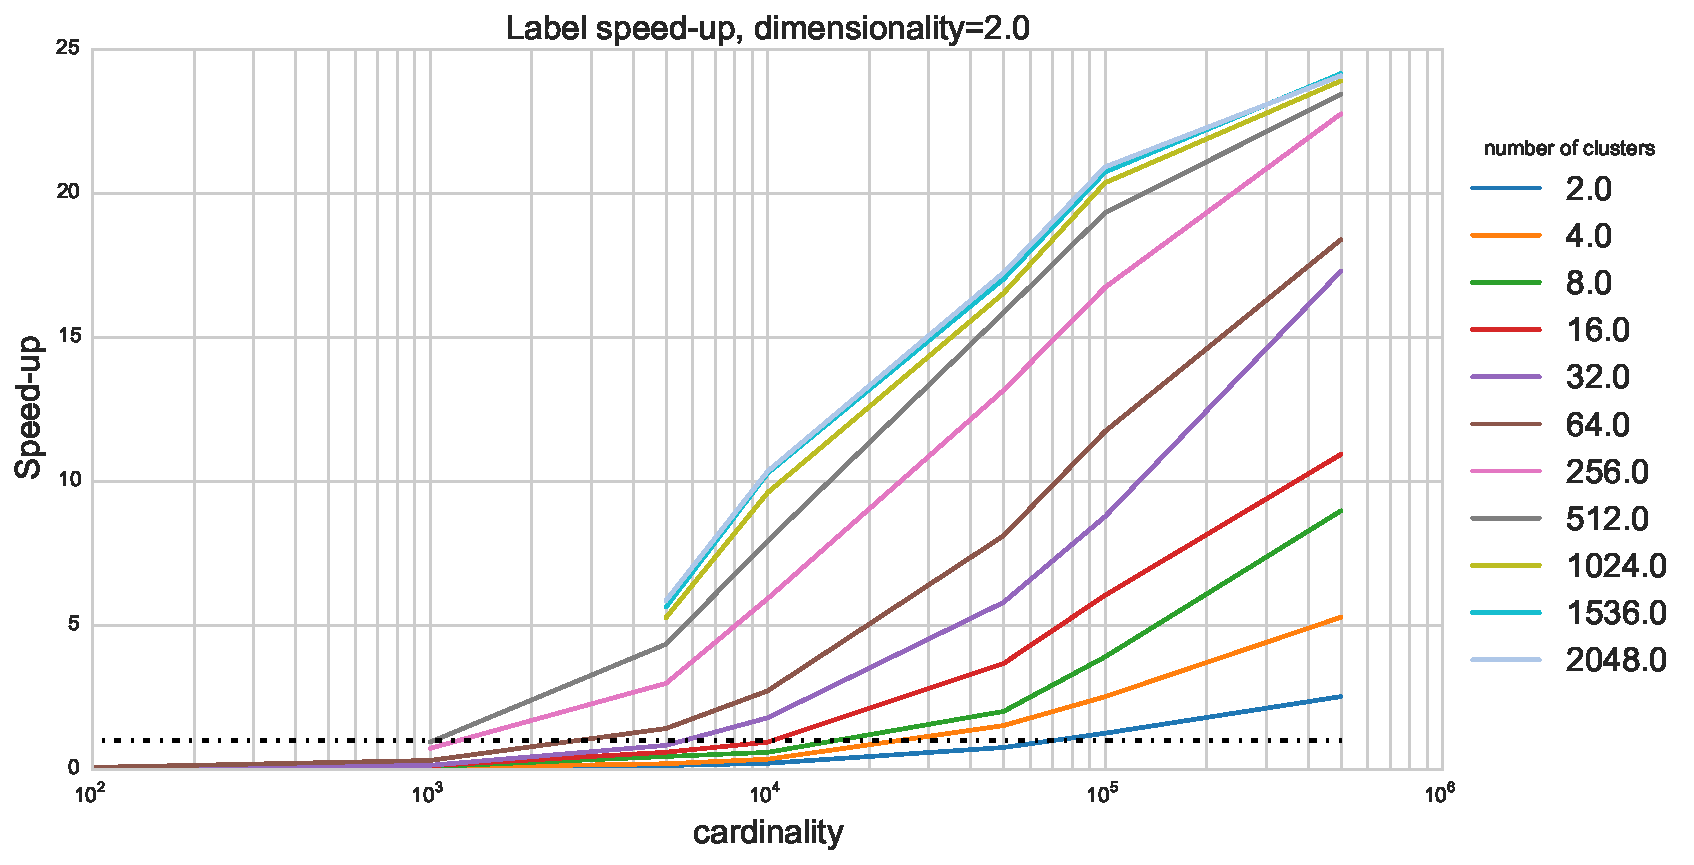
\includegraphics[width=\textwidth]{{{results/kmeans/fixed_dimensions/2.0}}}
    \caption{Speed-up of the labeling phase for datasets of 2 dimensions and varying cardinality and number of clusters. The dotted black line represents a speed-up of one.}
    \label{fig:kmeans dim 2}
\end{figure}

However, as the number of dimensions increases (observe Fig. \ref{fig:kmeans dim 200}), the speed-up increases until a certain number of patterns and then decreases.
Here, the initial number of patterns for which there is a speed-up is lower than in the low dimensionality case and the number of clusters plays less an influence on the speed-up.
It is believed that the reason for this is related to the implementation itself.
The current parallel implementation does not use shared memory, which is fast.
As such, for every computation, each thread fetches the relevant data from global memory which is significantly slower.
As the number of dimensions increases, the amount of data that each thread must fetch also increases.
Furthermore, since the number of dimensions affects both data points and centroids, if the number of dimensions increases by 2 the number of fetches to memory increases by 4.
So, the speed-up increases with the dataset complexity until a point where the number of fetches to memory starts having a very significant effect on the execution time, decreasing the speed-up close to $50\%$.

% As it stands, this implementation of K-Means excels in low-dimensional datasets with a high number of centroids.
% Good performance on a high number of centroids is a desireble thing given the overall context 

\begin{figure}[hbtp]
    \centering
    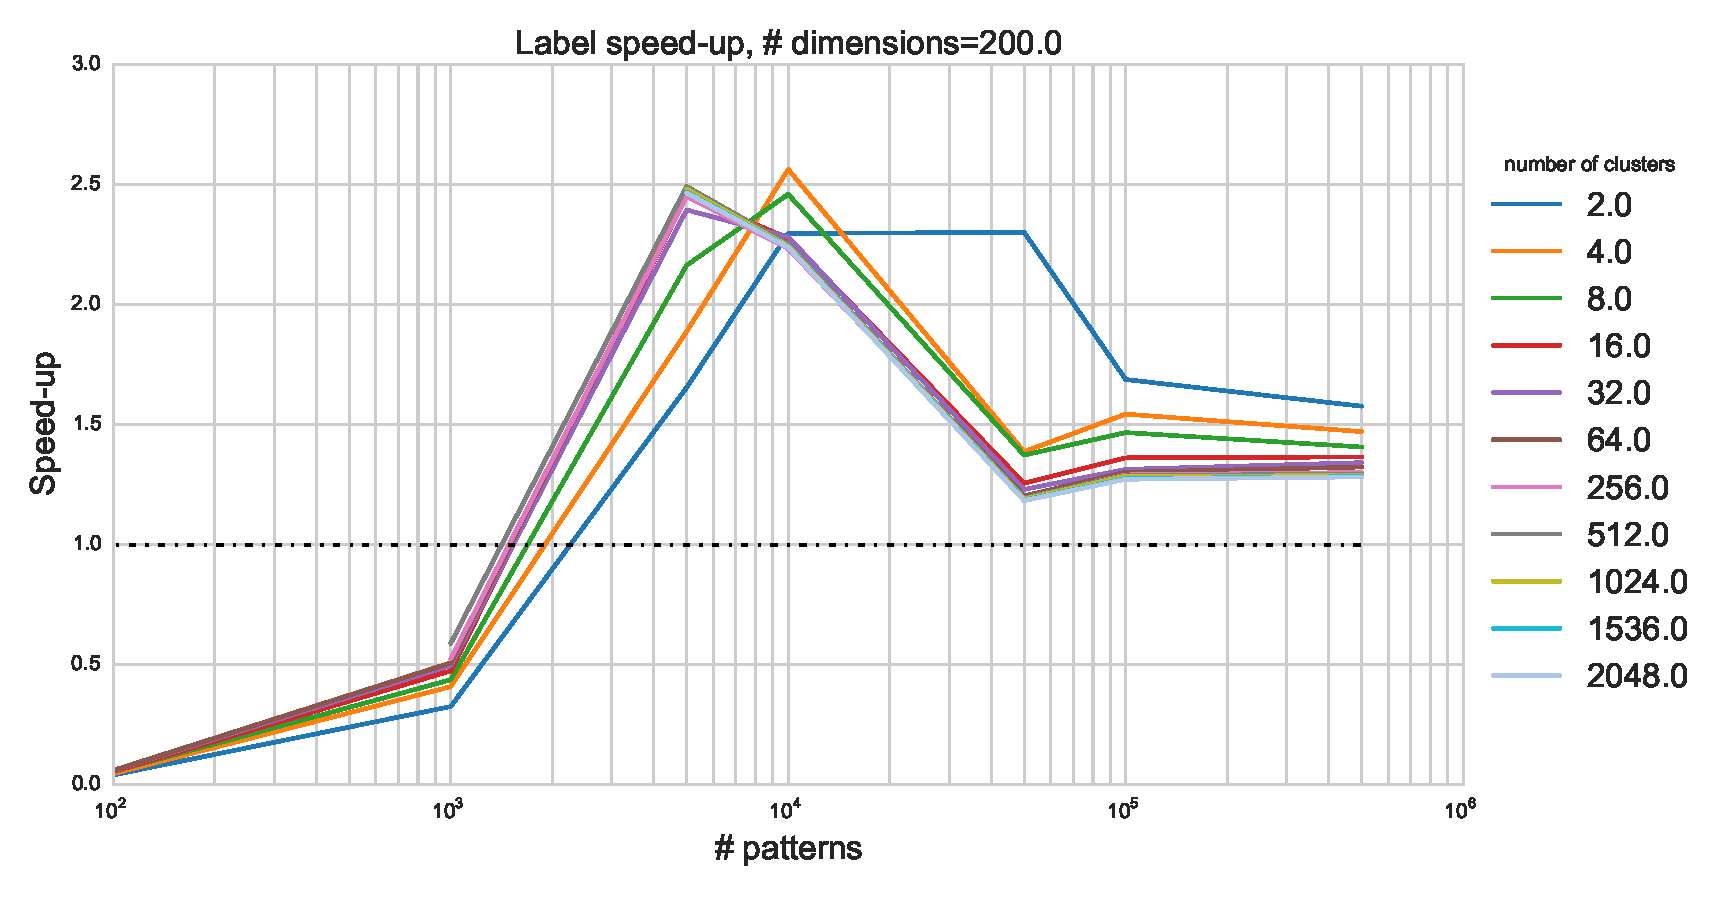
\includegraphics[width=\textwidth]{{{results/kmeans/fixed_dimensions/200.0}}}
    \caption{Speed-up of the labeling phase for datasets of 200 dimensions and varying cardinality and number of clusters. The dotted black line represents a speed-up of one.}
    \label{fig:kmeans dim 200}
\end{figure}

\subsection{Effective bandwidth and computational throughput}
% check devblogs.nvidia.com/parallelforall/how-implement-performance-metrics-cuda-cc/

Effective bandwidth and throughput are two useful metrics to measure the efficiency of CUDA programs.
The effective bandwidth was computed by summing the times of transferring data to and fro the device divided by the total amount of data transfered and is usually represented in GBytes/s.
The computational throughput is usually represented in GFLOP/s (Giga-FLoating-point OPerations per second).
These metrics were computed from the results and a statistical overview is presented in Table \ref{tab:kmeans performance metrics}.
The results refer only to the labeling phase to make a fair comparison between CPU and GPU, although considering both phases would not alter significantly the results since the update phase represents a small fraction of the computational complexity.
The computational throughput of the GPU is more than 3 times higher than that of the CPU, on average.
However, it is interesting to note that the minimum GPU throughput is significantly lower than the CPU.
This is because of what was seen in previous sections, where the dataset complexity is too low for the overhead associated with using the GPU to outweigh the benefit of the parallel computation.
Furthermore, it should be noted that the effective metrics of the GPU are well below the maximum theoretical presented in the device specifications, which are a bandwidth of 288 GB/s and a throughput of 4.29 TFLOP/s.
This suggests that the GPU is underused on the presented test cases. % usage on the presented test cases is still underused.

\begin{table}[ht]
\centering
\caption{Effective bandwidth and computational throughput of labeling phase computed from results taken from running K-Means over datasets whose complexity ranged from $100$ to $10 \: 000 \: 000$ patterns, from $2$ to $1000$ dimensions and from $2$ to $2048$ centroids.}

\begin{tabular}{lrrr}
\toprule
{} &  GPU bandwidth [GB/s] &  GPU throughput [GFLOP/s] &  CPU throughput [GFLOP/s] \\
\midrule
mean             &         2.902388 &    3.655521 &        1.048632 \\
std              &         2.278465 &    4.510252 &        0.330869 \\
min              &         0.001433 &    0.003631 &        0.029959 \\
25\% percentile &         0.567006 &    1.547014 &        0.872651 \\
50\% percentile  &         2.892260 &    1.711037 &        1.179825 \\
75\% percentile  &         5.319831 &    4.168283 &        1.296973 \\
max             &         6.044631 &   21.915104 &        1.447981 \\
\bottomrule
\end{tabular}

\label{tab:kmeans performance metrics}
\end{table}

\subsection{Influence of the number of points per thread}

The number of patterns each thread processes (PPT) may influence performance as well.
To evaluate this hypothesis, several runs over the datasets of $500 \: 000$ patterns with different points per thread were executed.
A brief statistical analysis of the results is presented in Table \ref{tab:kmeans cuda ppt}.
The average speed-up almost doubled when executing 2 PPT.
For more than 2 PPT, the speed-up seemed to decrease with an increase of the number of PPT.
Since the labeling kernel was not optimized for reducing the number of memory calls when processing more than one PTT, the increase in speed-up may be justified by the reduced overhead of calling less blocks of threads.
The fraction of the threads that did not execute any patterns increased with the PPT, which may be the cause for the decrease of speed-up with an increase of PPT after 2.

\begin{table}[h]
\centering
\caption{Speed-up obtained in the labeling phase for different number of patterns per thread (PPT).}


\begin{tabular}{lrrrrr}
\toprule
{} &       {} 	   &   {} 		   &  \textbf{Speed-up}  & {} 		& {}\\
{} &       PPT = 1 &       PPT = 2 &       PPT = 4 &       PPT = 8 &      PPT = 16 \\
\midrule
mean  &   5.898964 &  10.147513 &   3.736146 &   3.113199 &   2.090518 \\
std   &   7.470687 &  13.379909 &   4.027777 &   3.007031 &   1.264650 \\
min   &   1.235194 &   2.457333 &   1.521486 &   1.376941 &   1.258223 \\
25\% percentile  &   1.300021 &   2.561924 &   1.584261 &   1.473213 &   1.363452 \\
50\% percentile  &   2.048436 &   2.704003 &   1.721874 &   1.572580 &   1.432653 \\
75\% percentile  &   4.828922 &   9.321841 &   2.063122 &   1.897468 &   1.696736 \\
max   &  24.151800 &  46.752640 &  12.845526 &   9.943271 &   4.952390 \\
\bottomrule
\end{tabular}

\label{tab:kmeans cuda ppt}
\end{table} % KMEANS RESULTS
\section{GPU MST}
\label{sec:gpu mst}

% From Sousa dissertation - the graphs he used and where he took them from
% The graph collection supplied provided by 9th DIMACS Implementation Challeng \footnote{http://www.dis.uniroma1.it/~challenge9/} include sparse graphs
% that depict the United States road network. These graphs are seen frequently in the recent literature. Furthermore, the OpenStreetMap’s \footnote{http://www.openstreetmap.org/} Portuguese road-network, provided by Geofabrik \footnote{http://download.geofabrik.de/europe/portugal.html} is included.

To test the performance of the GPU MST algorithm, several graphs were used.
Most of the graphs are United Stated road network graphs taken from the 9th DIMACS Implementation Challenge \footnote{http://www.dis.uniroma1.it/~challenge9/}.
Furthermore, graphs taken from co-association matrix of the second step of EAC were used.
This is important because, as will become clear, the graphs within the EAC paradigm have different characteristics.
All the tests were performed on machine Bravo.
The average speed-up obtained by using the GPU version over the sequential one is presented in Table \ref{tab:mst speedup}.
Characteristics of the different graphs are also shown so as to illustrate what variables influence the speed-up obtained.
It should be noted that a speed-up below 0 is actually a slow-down and its absolute value corresponds to the speed-up of the sequential version relative its GPU counterpart.

\begin{minipage}[h]{\hsize}
	\centering
	\captionof{table}{Average speed-up of the GPU MST algorithm for different data sets, sorted by number of edges.}
\begin{tabular}{lrrrrr}
\toprule
Data set &  No. vertices &   No. edges &     Speed-up \footnote{Average speed-up from 10 rounds of executing the algorithm on each graph.} &  No. edges / vertex & Memory [MBytes]\\
\midrule

NY                           &      264347 &    730100 &  0.77 &          2.76 &    7.59 \\
BAY                          &      321271 &    794830 &  0.79 &          2.47 &    8.52 \\
COL                          &      435667 &   1042400 &  0.99 &          2.39 &   11.28 \\
FLA                          &     1070377 &   2687902 &  1.39 &          2.51 &   28.67 \\
NW                           &     1207946 &   2820774 &  1.45 &          2.34 &   30.74 \\
NE                           &     1524454 &   3868020 &  1.56 &          2.54 &   41.14 \\
CAL                          &     1890816 &   4630444 &  1.58 &          2.45 &   49.75 \\
LKS                          &     2758120 &   6794808 &  1.69 &          2.46 &   72.88 \\
E                            &     3598624 &   8708058 &  1.80 &          2.42 &   93.89 \\
W                            &     6262105 &  15000000 &  1.94 &          2.39 &  163.13 \\
Coassoc 50k \footnote{Co-association matrix of a 100 partition ensemble produced from a mixture of 6 Gaussians with $50 \: 000$ patterns, using the rule sk=sqrt\_2 th=30\%.} 							   &       50000 &  30296070 &  0.20 &        605.92 &  231.52 \\
CTR                          &    14000000 &  34000000 &  2.09 &          2.43 &  365.82 \\

\bottomrule
\end{tabular}
\label{tab:mst speedup}
\end{minipage}

% note on the memory usage
Although all the graphs presented in Table \ref{tab:mst speedup} occupy significantly less memory than the available in the used machine, the processing of bigger graphs is not possible.
The reason for this is that between in each iteration two graphs have to be held in memory: the initial and the contracted.
Moreover, the space occupied by the contracted graph will depend on the characteristics of the graph.

% speed-ups are possible, contrast with original paper
The results clearly show that it is possible to obtain speed-ups for computing a MST.
This speed-up seems to increase with the size of the graph, with the notable exception of the graph from the EAC context.
A note should be made here to bring to attention the contrast between these results and those presented by \citet{Sousa2015}.
The speed-ups observed here are less than those reported by \citet{Sousa2015}.
This is believed to be related with the technology stack used and this topic has been discussed in more depth in chapter \ref{chapter:methodology}.
To understand how different parameters affect the speed-up of the algorithm, Table \ref{tab:mst corr} presents the correlation matrix of these variables.

\begin{table}[h]
\centering
 \caption{Cross-correlation between several characteristics of the graphs and the average speed-up.}
\begin{tabular}{lrrr}
\toprule
{} &  No. vertices &   No. edges &        No. edges / vertex \\
\midrule
Average speed-up             &    0.692 &  0.081 &         -0.654 \\
\bottomrule
\label{tab:mst corr}
\end{tabular}
\end{table}

%TODO run MST algorithm with more graphs of different characteristics
% what are the variables that influence speed-up
The row corresponding to the average speed-up is of special relevance.
One can observe that the parameters most correlated with the speed-up are the number of vertices and the number of edges per vertex (EPV).
The correlation matrix suggests that as one increases the number of vertices, the speed-up will also increase.
In fact, if no graphs from the EAC context were present in the results, the same would apply to the number of edges, since the EPV would very similar.
The reason for this is that speed-ups from parallelism are more salient when applied to big data sets, so that the speed-up of the computation itself outweighs the overhead associated with communication between host and device.
The EPV is the other parameter that shows has highest (inverse) correlation with the speed-up.
This suggests that the relationship between the number of edges and the number of vertices in the graph actually plays a big role in deciding if there will be a speed-up.

% why, programatically, there is slow-down
The underlying reason for the poor performance of graphs with high EPV ratio is believed to be that, since the parallel computation is anchored to vertices, the workload per vertex is higher than if the graph had a low ratio.
Accordingly, the workload per vertex is higher from the beginning and can increase significantly as the algorithm progresses.
Besides, the workload can become highly unbalanced with some threads having to process hundreds of thousands of edges while others only a few thousands, which translates threads not doing any computation when waiting for the others.

% connection with original paper
The original source \cite{Sousa2015} of the algorithm doesn't address graphs with a EPV as high as presented here.
In that sense, the results here complement those of the original source and suggest an increase in EPC translates in the decrease in speed-up.
Still, more in-depth studies should be made.

% connection with EAC
Within EAC paradigm, this algorithm is of little contribution.
The most obvious reason is that the EAC method would actually be slower if this algorithm was used.
Still, even considering that speed-ups like those reported in literature were possible for EAC co-association graphs, the algorithm requires a double redundancy of edges (which effectively doubles the necessary memory to hold a graph) and at any iteration the device must be able to hold two distinct graphs (the initial and the contracted).
For these reasons, the device memory (which typically is smaller than the host memory) would confine the EAC method to small input data sets. 

% The underlying reason for this is believed to be that the number of edges to node ratio of these graphs is low compared to that typically seen in co-associations matrix, even when using a prototype subset of the original matrix.
% The parallel version of the final step of EAC showed a slowdown relative to its sequential counterpart.
% This slowdown is related with the performance of the MST algorithm.
% The implementation of the algorithm was tested in some of the same graphs as those reported in \cite{Sousa2015} and revealed a speedup.
% However, when using the this MST solver on the target graphs (the co-association matrices) not only there was no speedup, but a significantly slowdown was observed, reaching up to nine times slower.
 % GPU MST RESULTS
\section{Building the co-association matrix with different sparse formats}
\label{sec:spare building}

The purpose of this section is to present brief results concerning the time that took to build a co-association matrix for different types of matrices.
The ensemble from which the co-association matrices are built has 100 partitions and was produced from a mixture of 6 Gaussians with 5000 patterns.
Only the upper triangular (condensed) matrix was built.
The types of matrices under test are: fully allocated (a "normal" matrix), LIL, DOK, CSR, an optimized fully allocated and the proposed EAC CSR.
The SciPy's LIL, DOK and CSR implementations were used.
All tests were executed in machine Bravo.

The time that took to update the first partition and the total time were recorded for the different types of matrix.
The results are presented in Table \ref{tab:coassoc build sparse} and also in Fig. \ref{fig:coassoc build sparse}.
For the CSR format only the first partition was updated, since it took a very long time to update just the first partition.
A rough estimate for the time it would take to update the whole matrix is around 15 hours, 100 times the time it took to update the first partition.
Observing the other timings, and for the exception of the EAC CSR matrix, this estimate should not be too far off.
The reason that the first partition update of the EAC CSR matrix was so much faster is that it only requires a simple copy of the partition to the data structure.

It is clear from the results that the optimized versions are much faster than any of the others.
These results focus on providing a justification for the design and implementation of a novel method of building the co-association matrix: a fully allocated matrix consumes too much memory but available sparse implementations are too slow.
For this purpose a small dataset as the one used suffices to demonstrate this point.
The difference between the two optimized versions will become clearer on future sections, where a more thorough study covering a wider spectrum of datasets is presented. 


\begin{table}[h]
\centering
 \caption{Execution times for computing the condensed co-association matrix using different matrix strategies.}
\begin{tabular}{crr}
\toprule
  Matrix type (condensed) &  Time 1st partition [s] &  Time ensemble [s] \\
\midrule
 Optimzed Fully allocated &                 0.001 &              0.139 \\
                  EAC CSR &                 0.004 &              1.470 \\
          Fully allocated &                 0.855 &             96.000 \\
                      LIL &                 5.390 &            614.000 \\
                      DOK &                12.500 &           1535.000 \\
                      CSR &               548.000 &                - \\
\bottomrule
\end{tabular}
\label{tab:coassoc build sparse}
\end{table}



\begin{figure}[hbtp]
\centering
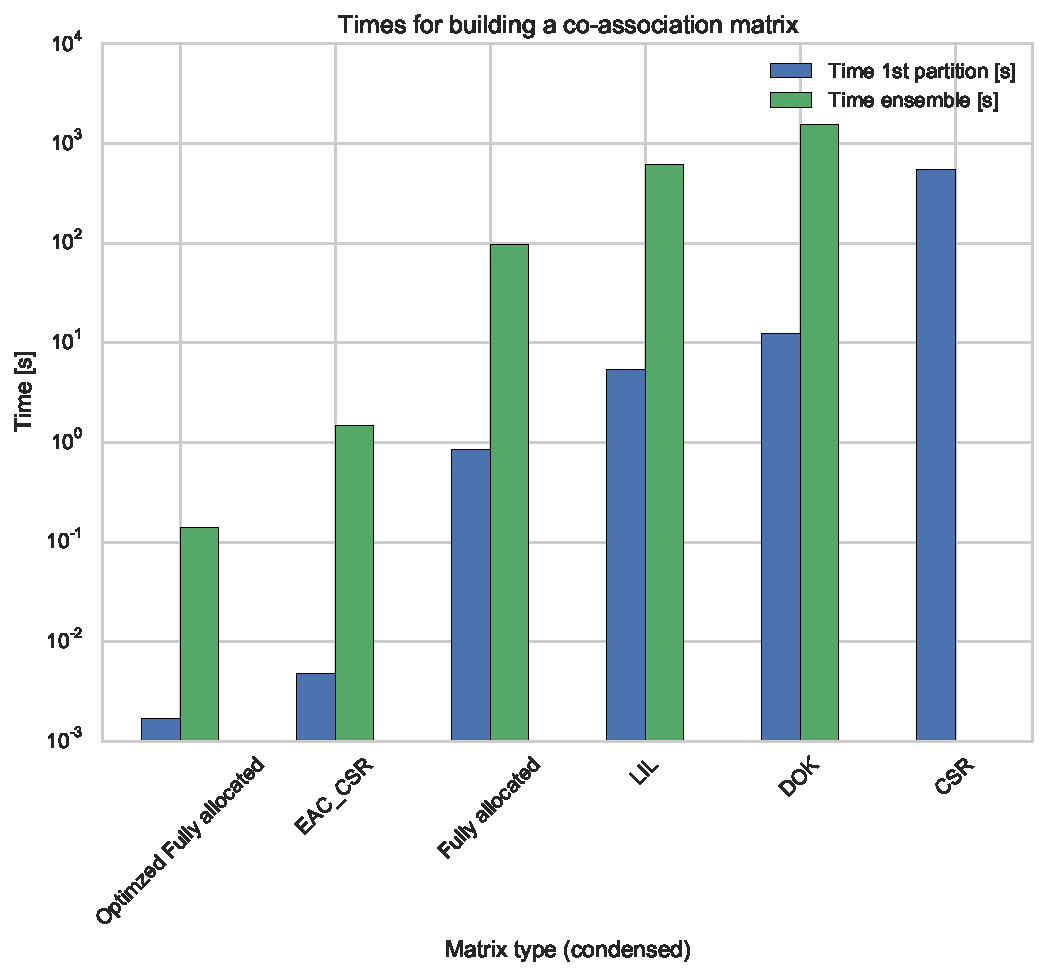
\includegraphics[scale=0.6]{results/eac_sparse_build/coassoc_build_bar}
\caption{Execution times for computing the condensed co-association matrix using different matrix strategies.}
\label{fig:coassoc build sparse}
\end{figure} % SPARSE BUILDNG RESUTLS
\section{EAC Validation}
\label{sec:eac validation}

The present section aims to provide results showing that the proposed methods do not alter the overall quality of the results.
With this in mind, the results of original version of EAC, implemented in Matlab, are compared with those of the proposed solution.
Several small data sets, chosen from the data sets used by \citet{Lourenco2010}, were processed by the two versions of EAC.
All these data sets were taken from the UCI Machine Learning Repository. %TODO add ref
Furthermore, since the generation of the ensemble is probabilistic and can change the results between runs, the proposed version is processed with the ensembles created by the original version as well.
This guarantees that the combination and recovery phases of EAC, which are deterministic when using SL, are equivalent to the original.
All data in this section refers to processing done in machine Alpha.

Table \ref{tab:validation error acc} presents the difference between the accuracies of the two versions.
Analyzing these results, it is apparent that the difference is minimal.
It should be noted at this point that the original implementation always maps the dissimilarities of the co-association matrix to the range $\left [ 0 , 1 \right ]$.
This forces the co-association matrix to have a floating point data type.
However, since the number of partitions used is usually less than 255, the proposed version uses unsigned integers of 1 byte to reduce the used memory considerably.
The differences in accuracy are thought to come from rounding differences of the two frameworks used and from this difference in data type.






\begin{table}[h]
\centering
\caption{Difference between accuracies from the two implementations of EAC, using the same ensemble. Accuracy was measured using the H-index.}

\begin{tabular}{lll}
\toprule
Data set &      Accuracy & Accuracy (lifetime) \\
\midrule
breast\_cancer &  4.948755e-06 &      2.825769e-06 \\
ionosphere    &  1.652422e-06 &      1.452991e-06 \\
iris          &  3.333333e-06 &      3.333333e-06 \\
isolet        &  1.038861e-07 &      4.084904e-07 \\
optdigits     &  3.795449e-06 &      1.480513e-06 \\
pima          &  3.333333e-06 &      3.333333e-06 \\
pima\_norm     &  4.166667e-07 &      4.166667e-07 \\
wine\_norm     &  1.123596e-07 &      1.910112e-06 \\
\bottomrule
\end{tabular}

\label{tab:validation error acc}
\end{table}




% \begin{table}[h]
% \centering
% \caption{Speed-ups obtained in the combination and recovery phases of EAC, using the ensemble generated from the original EAC implementation.}

% \begin{tabular}{lll}
% \toprule
% Data set & Combination & Recovery \\
% \midrule
% breast\_cancer &   7.713564 &        15.22334 \\
% ionosphere    &   9.678288 &        20.12336 \\
% iris          &   14.25549 &         28.4751 \\
% isolet        &   5.500147 &        174.4283 \\
% optdigits     &   9.783604 &        53.21466 \\
% pima          &   85.21744 &        8.406726 \\
% pima\_norm     &   127.2274 &        12.89474 \\
% wine\_norm     &     8.0178 &        12.98206 \\
% \bottomrule
% \end{tabular}

% \label{tab:validation speedup comb rec}
% \end{table}

Table \ref{tab:validation speedup all} presents the speed-up of the proposed version over the original one.
It is clear that speed-up is obtained in all phases of EAC, often by an order of magnitude.
This result, combined with the demonstration that the differences in accuracy are negligible, show that the proposed algorithm performs well in small data sets.

\begin{table}[h]
\centering
\caption{Speed-ups obtained in the different phases of EAC, with independent production of ensembles.}

\begin{tabular}{lccllll}
\toprule
Data set &  No. patterns &  No. features & No. classes & Production & Combination & Recovery \\
\midrule
breast\_cancer &           683 &            10 &           2 &      50.43974 &   7.544247 &        15.83316 \\
ionosphere    &           351 &            34 &           2 &      21.86286 &   11.30883 &        19.97219 \\
iris          &           150 &             4 &           3 &      19.76525 &   14.49562 &        28.50479 \\
isolet        &          7797 &           617 &          26 &      7.010007 &   6.183124 &        206.2837 \\
optdigits     &          3823 &            64 &          10 &      17.30209 &    10.2096 &        53.02636 \\
pima          &           768 &             8 &           2 &      50.65624 &   141.4828 &        13.93502 \\
pima\_norm     &           768 &             8 &           2 &      54.25415 &   132.8632 &          14.355 \\
wine\_norm     &           178 &             4 &           3 &      22.92404 &   14.56994 &        25.27709 \\
\bottomrule
\end{tabular}

\label{tab:validation speedup all}
\end{table}


 % EAC VALIDATION RESUTLS
\section{EAC}
\label{sec:eac results}

This section will present thorough results concerning several characteristics related to the EAC method.
These were the timings of the different parts, how the number of patterns and the different $K_{min}$ rules affected the sparsity of the co-association matrix, the typical number of associations per cluster in each rule, the growth of the number of associations with the different parameters, among others.
Two 2-dimensional 10 million pattern mixtures of 6 Gaussians were generated.
A variation of the number of dimensions has more interest in the performance characteristics of the production phase.
Since the production of the ensemble uses K-Means, detailed results can be found in section \ref{sec:parallel kmeans}.
One mixture has overlapping Gaussians and the other has not.
% The reasoning was that overlapping Gaussians might result in more associations per cluster.
The results contained in this section refer to the dataset with overlapping Gaussians, but the same overall patterns can be found in the other and the same conclusions can be drawn.

Different rules for computing the $K_{min}$, different co-association matrix formats and different approaches for the final clustering will be mentioned.
The different rules and their aliases are presented in Table \ref{tab:eac rules}.
The different formats for the co-association matrix are the \emph{full} (for fully allocated $n \times n$ matrix), \emph{full condensed} (for a fully allocated $\frac{n(n-1)}{2}$ array to build the upper triangular matrix), \emph{sparse complete} (for EAC CSR), \emph{sparse condensed const} (for EAC CSR building only the upper triangular matrix) and \emph{sparse condensed linear} (for EAC CSR condensed).
The different approaches for the final clustering are \emph{SLINK} \cite{Sibson1973}, \emph{SL-MST} (for using the Kruskal implementation in SciPy) and \emph{SL-MST-Disk} for the modified version that performs an external memory sort.

\begin{table}[h]
\centering
\caption{Different rules for computing $K_{min}$ and $K_{max}$. $n$ is the number of patterns and $sk$ is the number of patterns per cluster.}

\begin{tabular}{lcc}
\toprule
Rule &  $K_{min}$ &  $K_{max}$ \\
\midrule
\emph{sqrt}     & $\frac{\sqrt{n}}{2}$      & $\sqrt{n}$    \\
\emph{2sqrt}    & $\sqrt{n}$                & $2 \sqrt{n}$  \\
\emph{sk=sqrt2} & $sk = \frac{\sqrt{n}}{2}$ & $1.3 K_{min}$ \\
\emph{sk=300}   & $sk = 300$                & $1.3 K_{min}$ \\
\bottomrule
\end{tabular}

\label{tab:eac rules}
\end{table}

The experiment that generated the results of these section was set up as follows.
A large dataset was generated.
The dataset was sampled uniformly to produce a smaller dataset with the desired number of patterns.
A clustering ensemble was produced (production phase) for each of these smaller datasets and for each of the rules, using K-Means.
From each ensemble, co-association matrices of every applicable format were built (combination phase).
A matrix format was not applicable when the dataset complexity would make its correspondent co-association matrix too big to fit in main memory.
The final clustering (recovery phase) was also done for each of the matrix formats.
SLINK was used with fully allocated formats and the MST-based SL (SL-MST) and MST-based SL on external memory (SL-MST-disk) were executed with sparse matrices.
SL-MST was not executed if its space complexity was too big to fit in main memory.
Furthermore, the combination and recovery phases were repeated several times for smaller datasets for statistical relevant of the execution times, so as to make the influence of any background process less salient.
For big datasets, the execution times are big enough that the influence of background processes is negligible.

All results presented here originated from machine Bravo.

\subsection{Performance of production and combination phases}

The execution times for the production and combination phase can be observed in Figures \ref{fig:eac ensemble times}, \ref{fig:eac build rules} and \ref{fig:eac build matrices}, which allow the comparison between the different rules and the different matrix formats, respectively.
To avoid redundancy, only one matrix format is depicted to compare the execution times for the different rules and only one rule to compare the matrix formats.
The results of the other cases follow the same pattern.

These times are related with the $K_{min}$ parameter, whose evolution is presented in Fig. \ref{fig:eac kmin evo}.
Rules \emph{sqrt}, \emph{2sqrt} and \emph{sk=sqrt2} never intersect but rule $sk=300$ intersects all of them, finishing with the highest $K_{min}$.
Observing Fig. \ref{fig:eac build rules}, one can see the same tendency in the production execution time associated with the $sk=300$ rule and the inverse in the combination time.
A higher $K_{min}$ means more centroids for each K-Means run to compute, so it is not surprising that the execution time for computing the ensemble increases as $K_{min}$ increases.

\begin{figure}[hbt!]
    \centering
    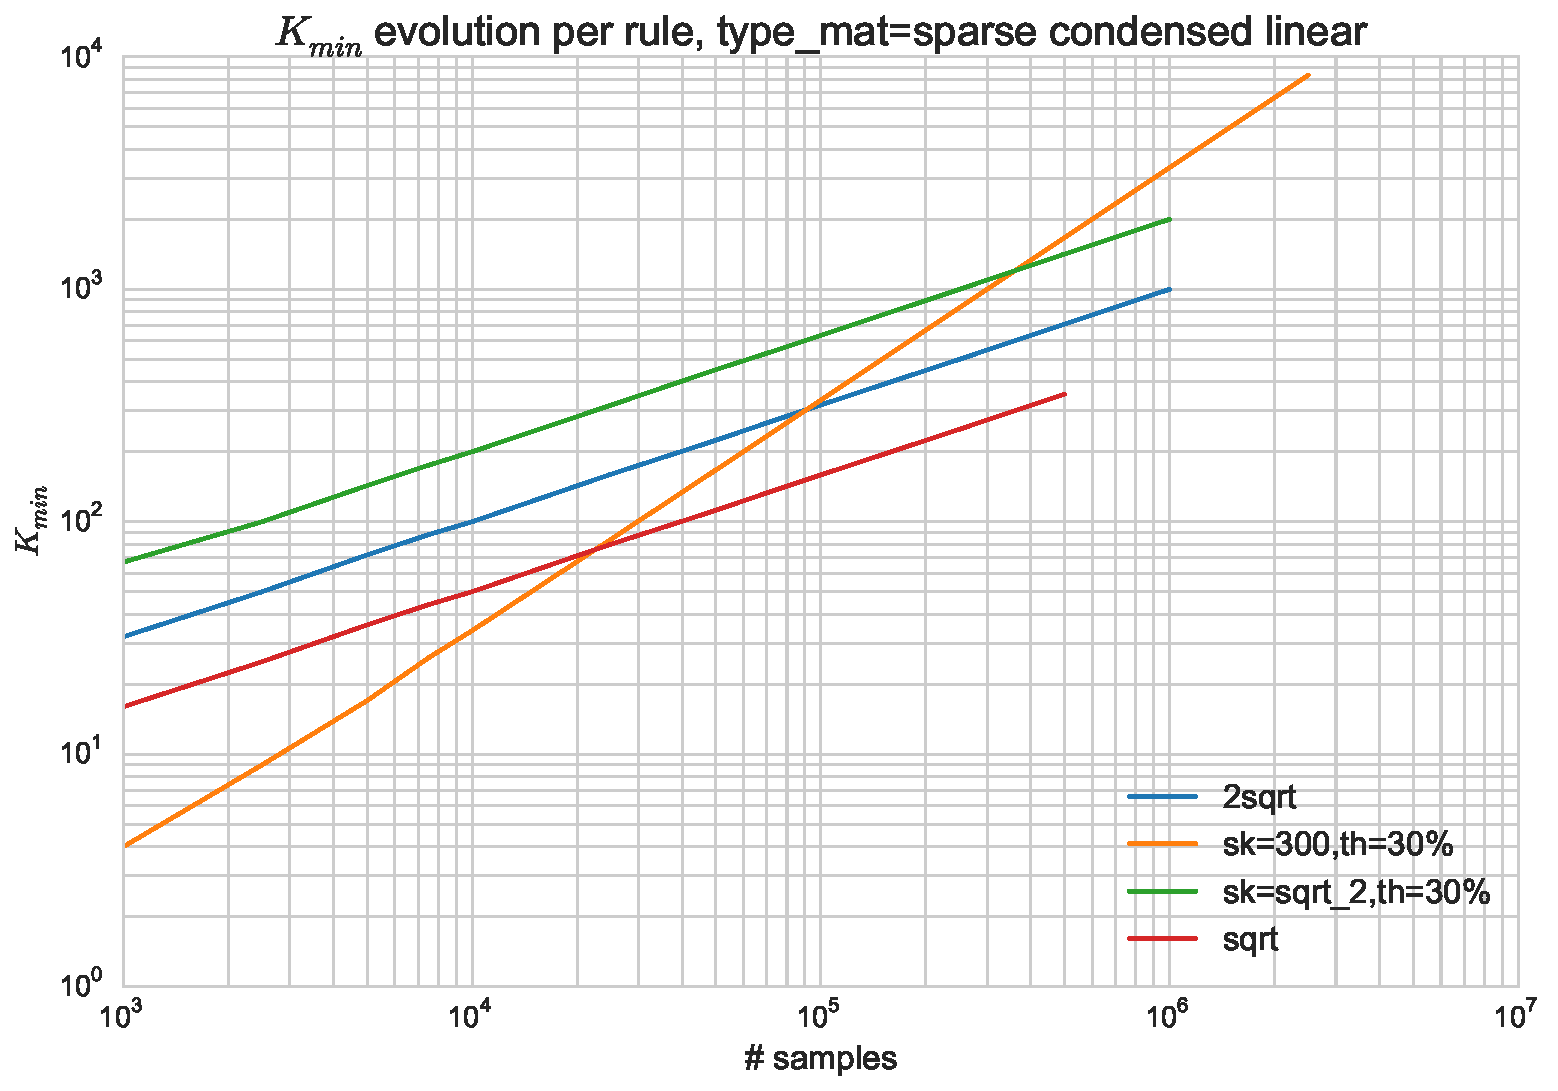
\includegraphics[width=0.6\textwidth]{{{results/eac/kmin_evolution}}}
    \caption{Evolution of $K_{min}$ with cardinality for different rules.}
    \label{fig:eac kmin evo}
\end{figure}

\begin{figure}[hbt!]
    \centering
    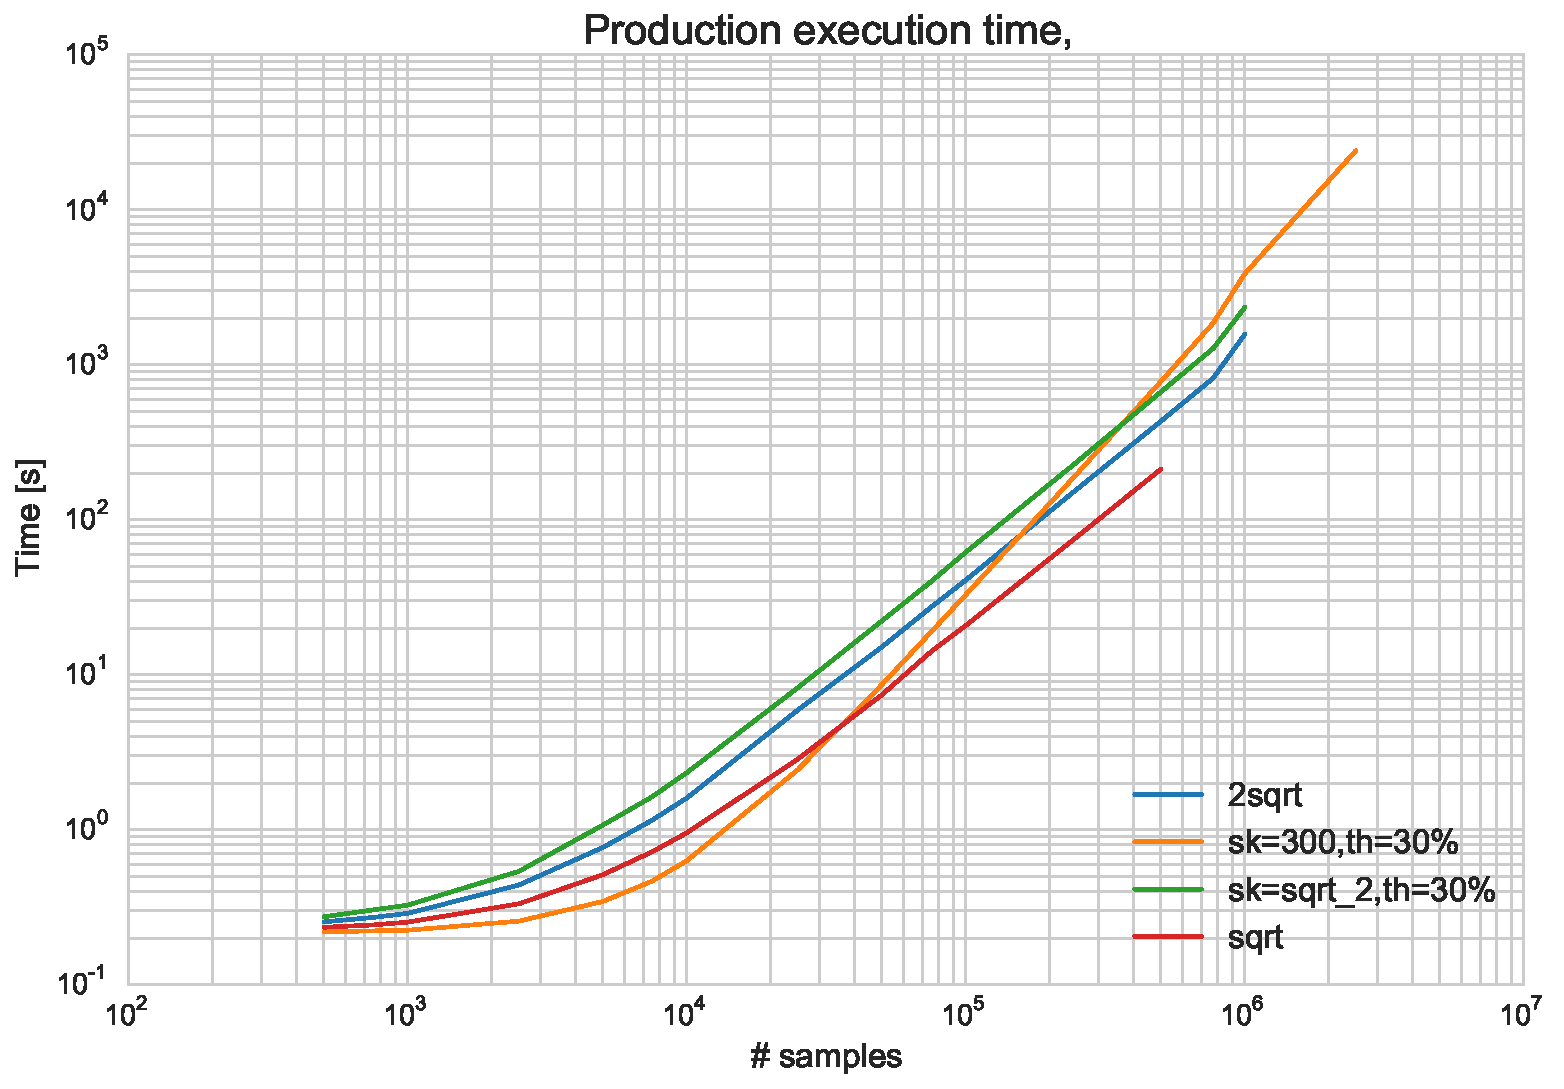
\includegraphics[width=0.6\textwidth]{{{results/eac/ensemble_time}}}
    \caption{Execution time for the production of the clustering ensemble.}
    \label{fig:eac ensemble times}
\end{figure}

In a previous section, the execution times for the combination phase had already been briefly presented when comparing different sparse formats.
Fig. \ref{fig:eac build matrices} shows the execution times on a longitudinal study for optimized matrix formats.
It is clear that the sparse formats are significantly slower than the fully allocated ones, specially for smaller datasets.
The \emph{full condensed} format usually takes close to half the time than the \emph{full} format, which is natural given that it performs half the operations.
Idem for the \emph{sparse condensed} formats compared to the \emph{sparse complete}.
The big discrepancy between the sparse and full formats is due to the fact that the former needs to do a binary search at each association update and needs to keep the internal sparse data structure sorted.


\begin{figure}[hbt!]
    \centering
    \includegraphics[width=0.6\textwidth]{{{results/eac/build_time/sparse_condensed_linear}}}
    \caption{Execution time for building the co-association matrix from ensemble with different rules.}
    \label{fig:eac build rules}
\end{figure}

\begin{figure}[hbt!]
    \centering
    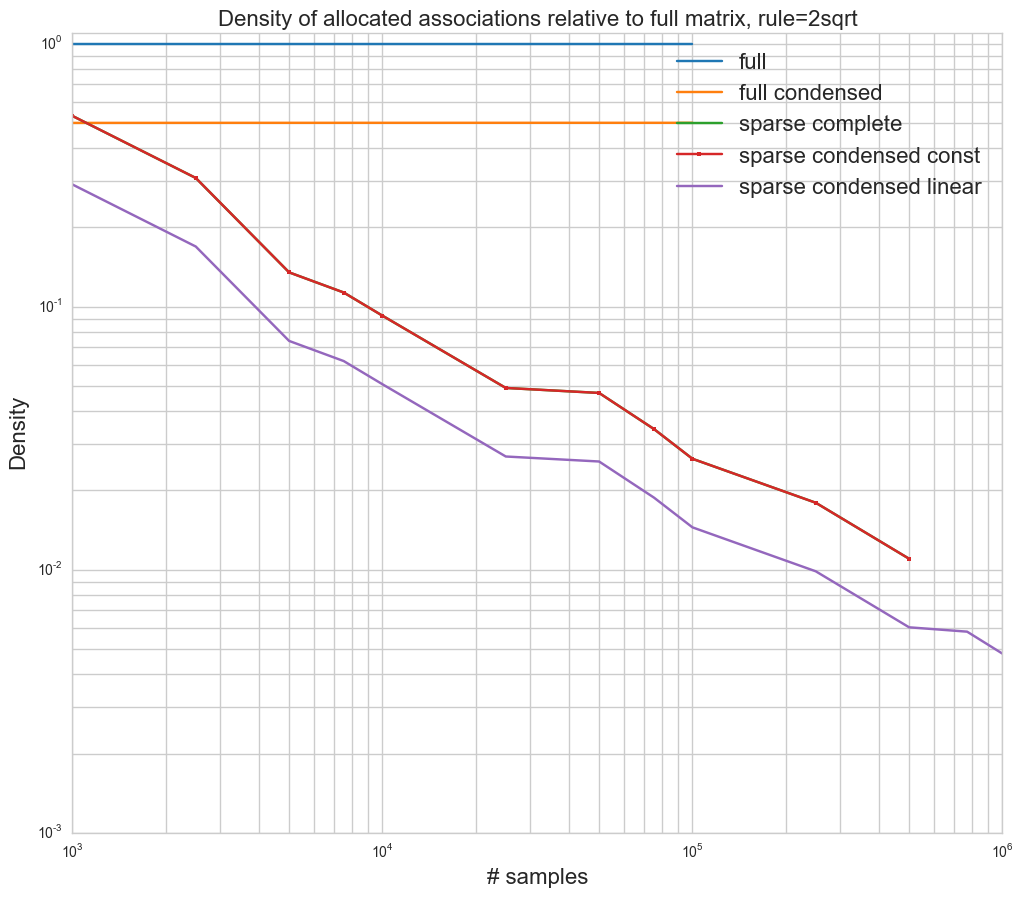
\includegraphics[width=0.6\textwidth]{{{results/eac/build_time/2sqrt}}}
    \caption{Execution time for building the co-association matrix with different matrix formats.}
    \label{fig:eac build matrices}
\end{figure}

\subsection{Performance comparison between SLINK, SL-MST and SL-MST-Disk}

The clustering times of the different methods of SL discussed previously (SLINK, SL-MST and SL-MST-Disk) are presented in Figures \ref{fig:eac sl}, \ref{fig:eac slink} and \ref{fig:eac sl-mst}.
The SL-MST-Disk method is significantly slower than any of the other methods.
This is expected, since it uses the hard drive which has very slow access times compared to main memory.
SL-MST is faster than SLINK, since it processes zero associations while SL-MST takes advantage of a graph representation and only processes the non-zero associations.
In resemblance to what happened with combination times, the condensed variants take roughly half the time has their complete counterparts.
This is expected, since SL-MST and SL-MST-Disk over condensed co-association matrices only process half the number of associations.
SLINK takes roughly the same time for every rule, which means $K_{min}$ has no influence, since SLINK processes the entire co-association matrix and $K_{min}$ only influences the number of non-zero associations.
The same rationale can be applied to SL-MST, where different rules can have significant influence over execution time, since they change the total number of associations.
As with the combination phase, the execution time referent to the \emph{sk=300} rule started with the greatest time and decreased with an increase in cardinality until it was the fastest.

\begin{figure}[hbt!]
    \centering
    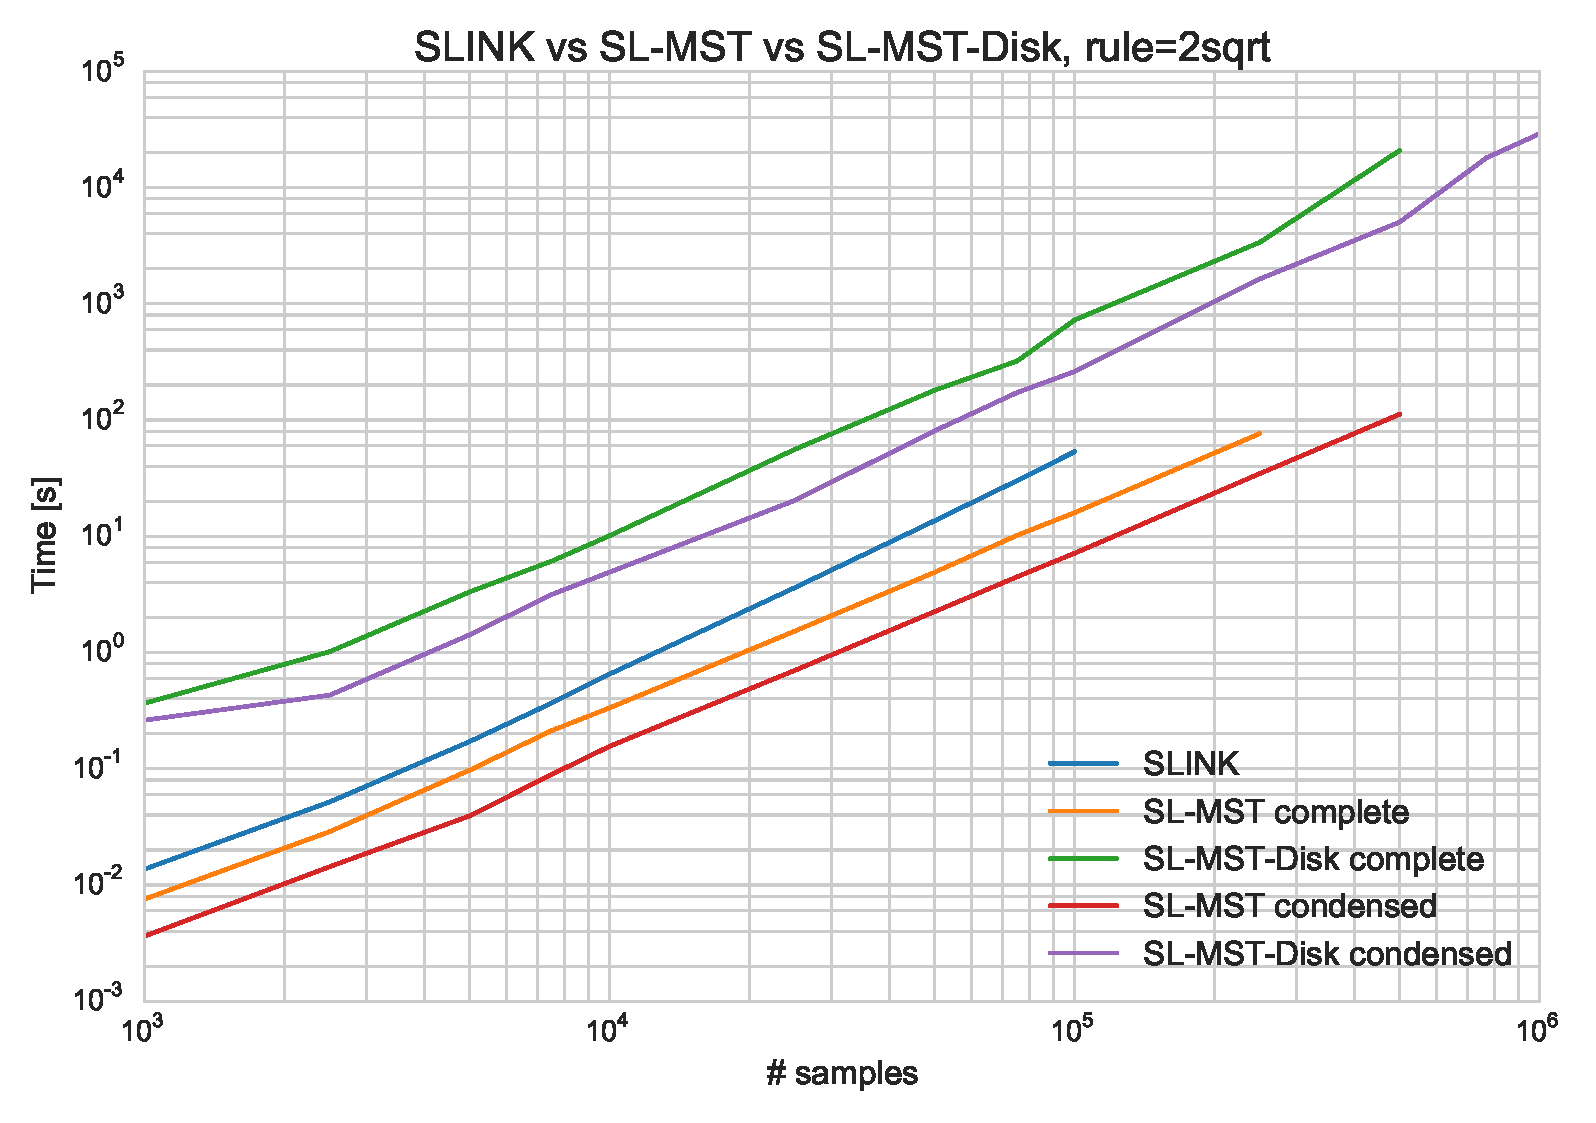
\includegraphics[width=0.6\textwidth]{{{results/eac/sl_time/slink_vs_sl-mst}}}
    \caption{Comparison between the execution times of the three methods of SL. SLINK runs over fully allocated condensed matrix while SL-MST and SL-MST-Disk run over the condensed and complete sparse matrices.}
    \label{fig:eac sl}
\end{figure}

\begin{figure}[hbt!]
    \centering
    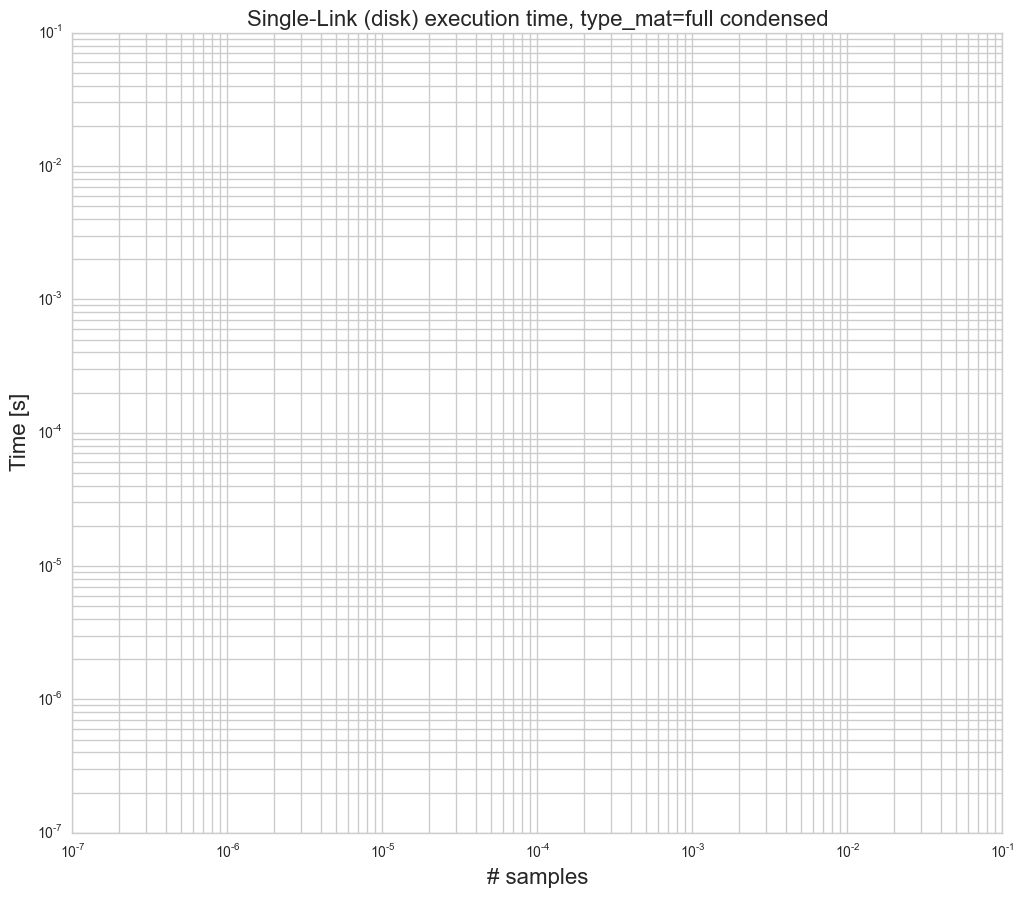
\includegraphics[width=0.6\textwidth]{{{results/eac/sl_mem_time/full_condensed}}}
    \caption{Comparison between the execution times of SLINK to different rules.}
    \label{fig:eac slink}
\end{figure}

\begin{figure}[hbt!]
    \centering
    \includegraphics[width=0.66\textwidth]{{{results/eac/sl_mem_time/sparse_condensed_linear}}}
    \caption{Comparison between the execution times of SL-MST for different rules.}
    \label{fig:eac sl-mst}
\end{figure}

\subsection{Performance of all phases combined}

The execution times of all phases combined are presented in Figures \ref{fig:eac total mem} and \ref{fig:eac total disk}.
The results are presented for the \emph{sparse condensed linear} format but the remaining results follow the same tendency.
It is interesting to note that, when using the SL-MST method in the recovery phase, the execution time for three of the rules do not differ much for large datasets.
This is due to a sort of balancing between a slowing down of the production phase and a speeding up of the combination and recovery phases as the $K_{min}$ increases at a higher rate for $sk=300$ than for other rules.
This is not observed for the $sqrt$ rule as $K_{min}$ is always low enough that the total time is always dominated by the combination and recovery phases.
The same does not happen when using the SL-MST-Disk method, as the total time is completely dominated by the recovery phase.
This is clear, since the results in Fig. \ref{fig:eac total disk} follow a pattern similar to that presented in Fig. \ref{fig:eac sl-mst}.


\begin{figure}[hbt!]
    \centering
    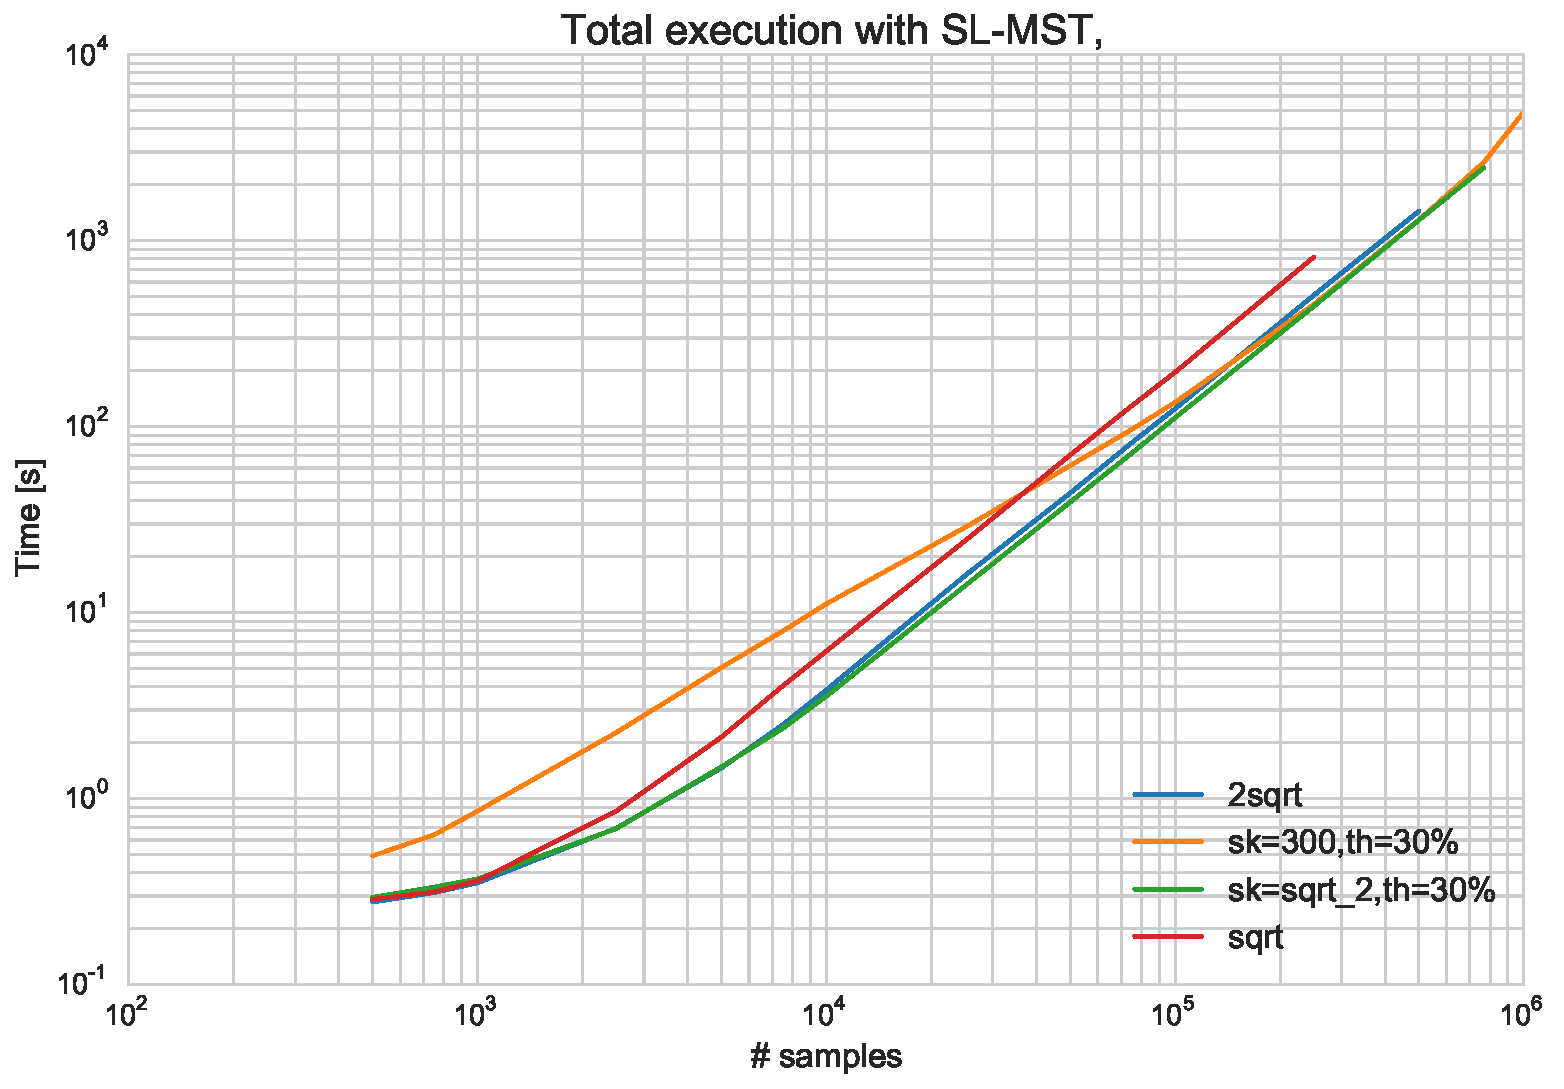
\includegraphics[width=0.6\textwidth]{{{results/eac/total_time_sl-mst}}}
    \caption{Execution times for all phases combined, using SL-MST in the recovery phase.}
    \label{fig:eac total mem}
\end{figure}

\begin{figure}[hbt!]
    \centering
    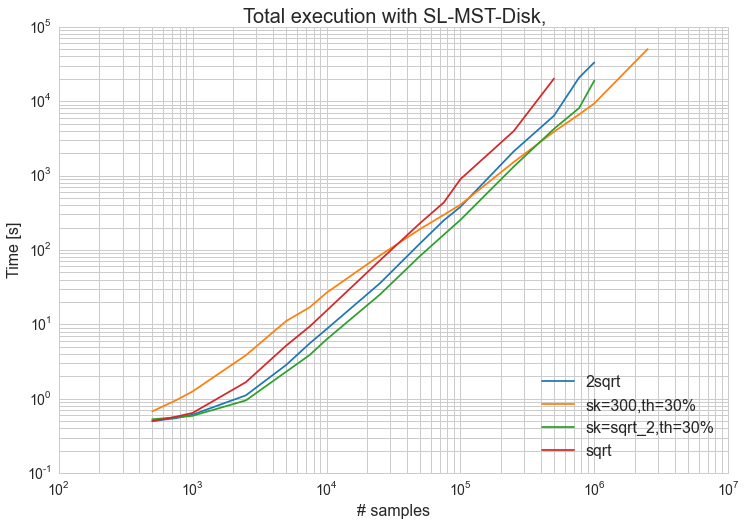
\includegraphics[width=0.66\textwidth]{{{results/eac/total_time_sl-mst-disk}}}
    \caption{Execution times for all phases combined, using SL-MST-Disk in the recovery phase.}
    \label{fig:eac total disk}
\end{figure}


\subsection{Analysis of the number of associations}

The sparse nature of EAC has been pointed out before and is clearer in Fig. \ref{fig:eac assoc density}.
This figure shows the association density, i.e. number of associations relative to the $n^2$ possible associations in a full matrix.
The \emph{full condensed} format as a constant density of $49.5\%$ and the density of \emph{sparse complete} is two times that of the \emph{sparse condensed} formats.
The overall tendency is for the density to decrease as the number of patterns of the dataset increases.
This is to be expected since the \emph{full} matrix grows quadratically.
Besides, it would be expected that the same associations would be grouped together more frequently in partitions and simply make previous connections stronger instead of creating new ones.
Results presented in Fig. \ref{fig:eac assocs per pattern}, which presents the number of associations per pattern, suggest that but it is only clear for the $sk=300$ rule.
The number of associations per pattern increases with the number of patterns of the dataset, with the notable exception of the \emph{sk=300} rule which increases until it reaches a certain limit and then stabilizes.
This is explained by the fact that this rule is based on setting a maximum constant number ($300$) of patterns in any given cluster, while in the other rules this number increases with the number of patterns.
The number of associations per pattern is not $300$ for the $sk=300$ rule because a pattern will be clustered with different neighbors in different partitions.
Still, the number of neighbors doesn't change enough that the number of associations per pattern increases boundlessly.
In fact, Fig. \ref{fig:eac assocs per pattern} suggests that the number of associations per pattern is around 3 times the upper bound on the number of patterns per cluster (strictly related to $K_{min}$).
This is clearer for $sk=300$, but if one would trace the the number of patterns divided by $K_{min}$ for each rule, a similar tendency would manifest.
\citet{Lourenco2010} reported that, on average, \"the overall contribution of the clustering ensemble (including unbalanced clusters) duplicates the co-associations produced in a single balanced clustering with Kmin clusters\".
The spectrum of datasets evaluated regarding number of patterns was smaller than that evaluated in the present work.
The present results suggest a slightly higher value.
So, the decrease in density is more related with the quadratic growth of the \emph{full} matrix in contrast with a linear growth of the number of associations.

\begin{figure}[hbt!]
    \centering
    \includegraphics[width=0.6\textwidth]{{{results/eac/assoc_density/sparse_condensed_linear}}}
    \caption{Density of associations relative to the full co-association matrix, which hold $n^2$ associations.}
    \label{fig:eac assoc density}
\end{figure}

\begin{figure}[hbt!]
    \centering
    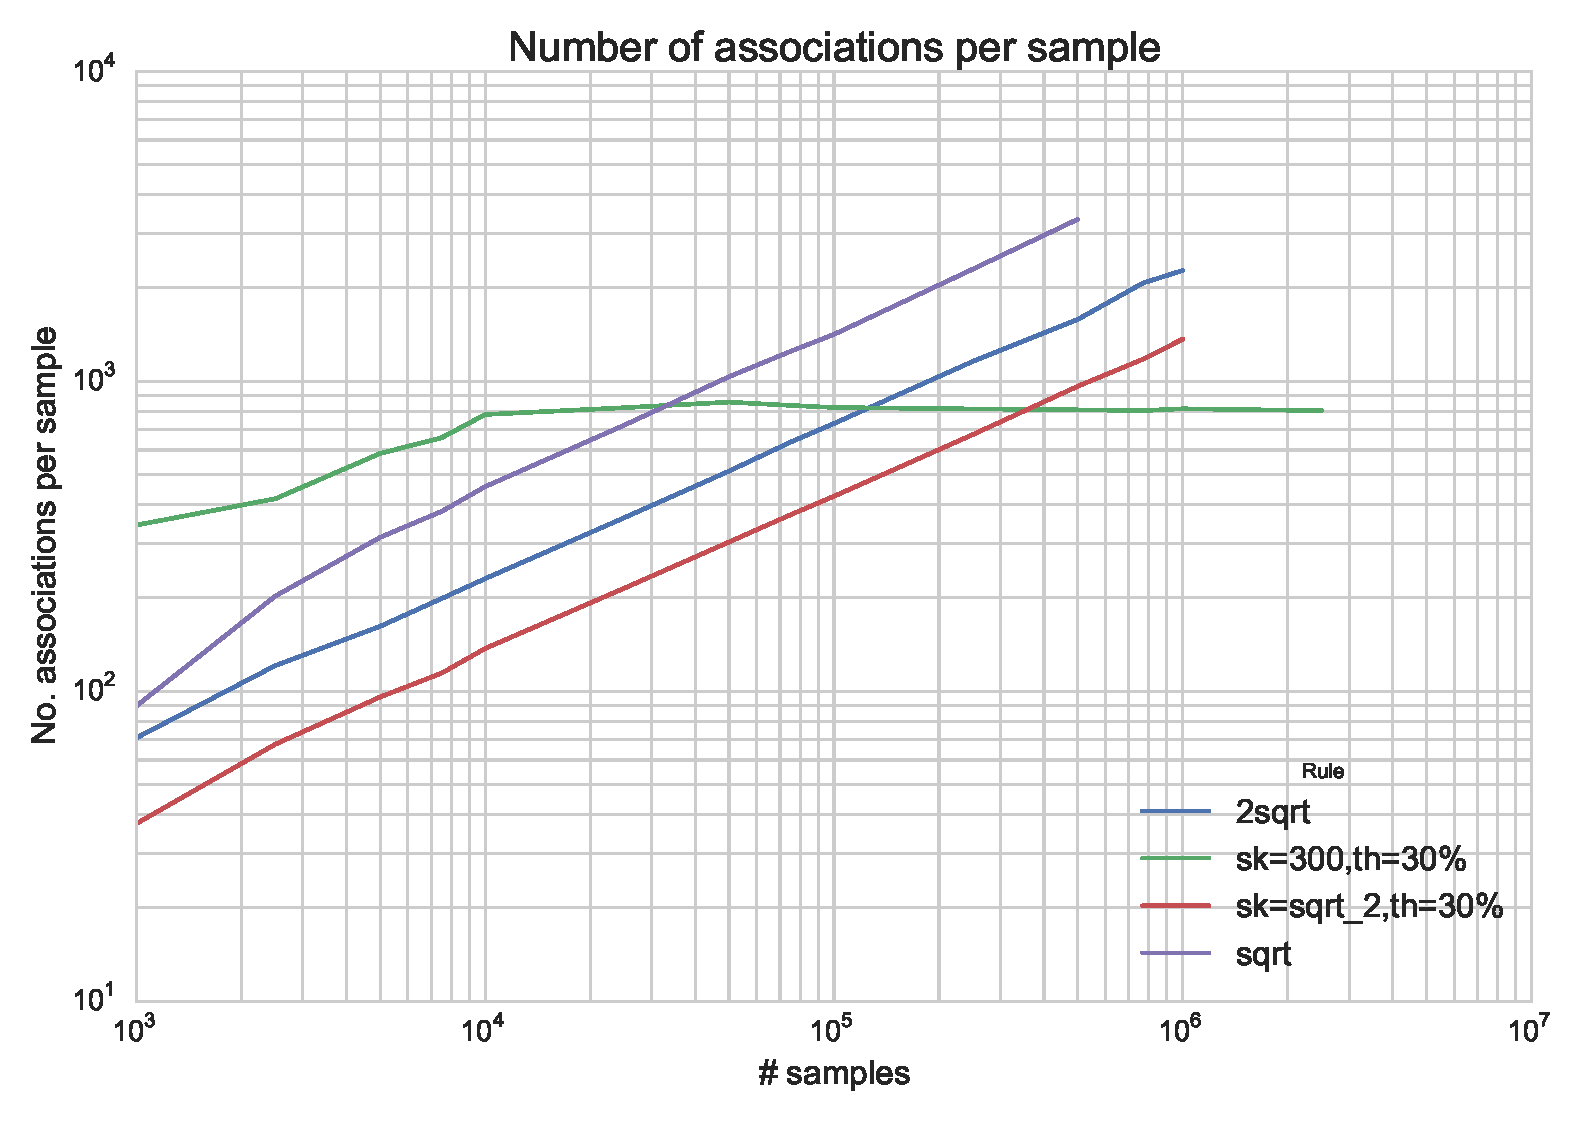
\includegraphics[width=0.6\textwidth]{{{results/eac/assocs_per_sample}}}
    \caption{Evolution of the total number of associations divided by the number of patterns according to the different rules.}
    \label{fig:eac assocs per pattern}
\end{figure}

Predicting the number of associations before building the co-association matrix is useful for coming up with combination schemes that are both memory and speed efficient.
It was stated before that the biggest cluster size in any partition of the ensemble is a good parameter for this end.
Fig. \ref{fig:eac max assocs per bgs} presents the relationship between the biggest cluster size and the maximum number of associations of any pattern.
These ratio increases with the number of patterns in the beginning, but as the number of patterns increases it never goes over 3.

\begin{figure}[hbt!]
    \centering
    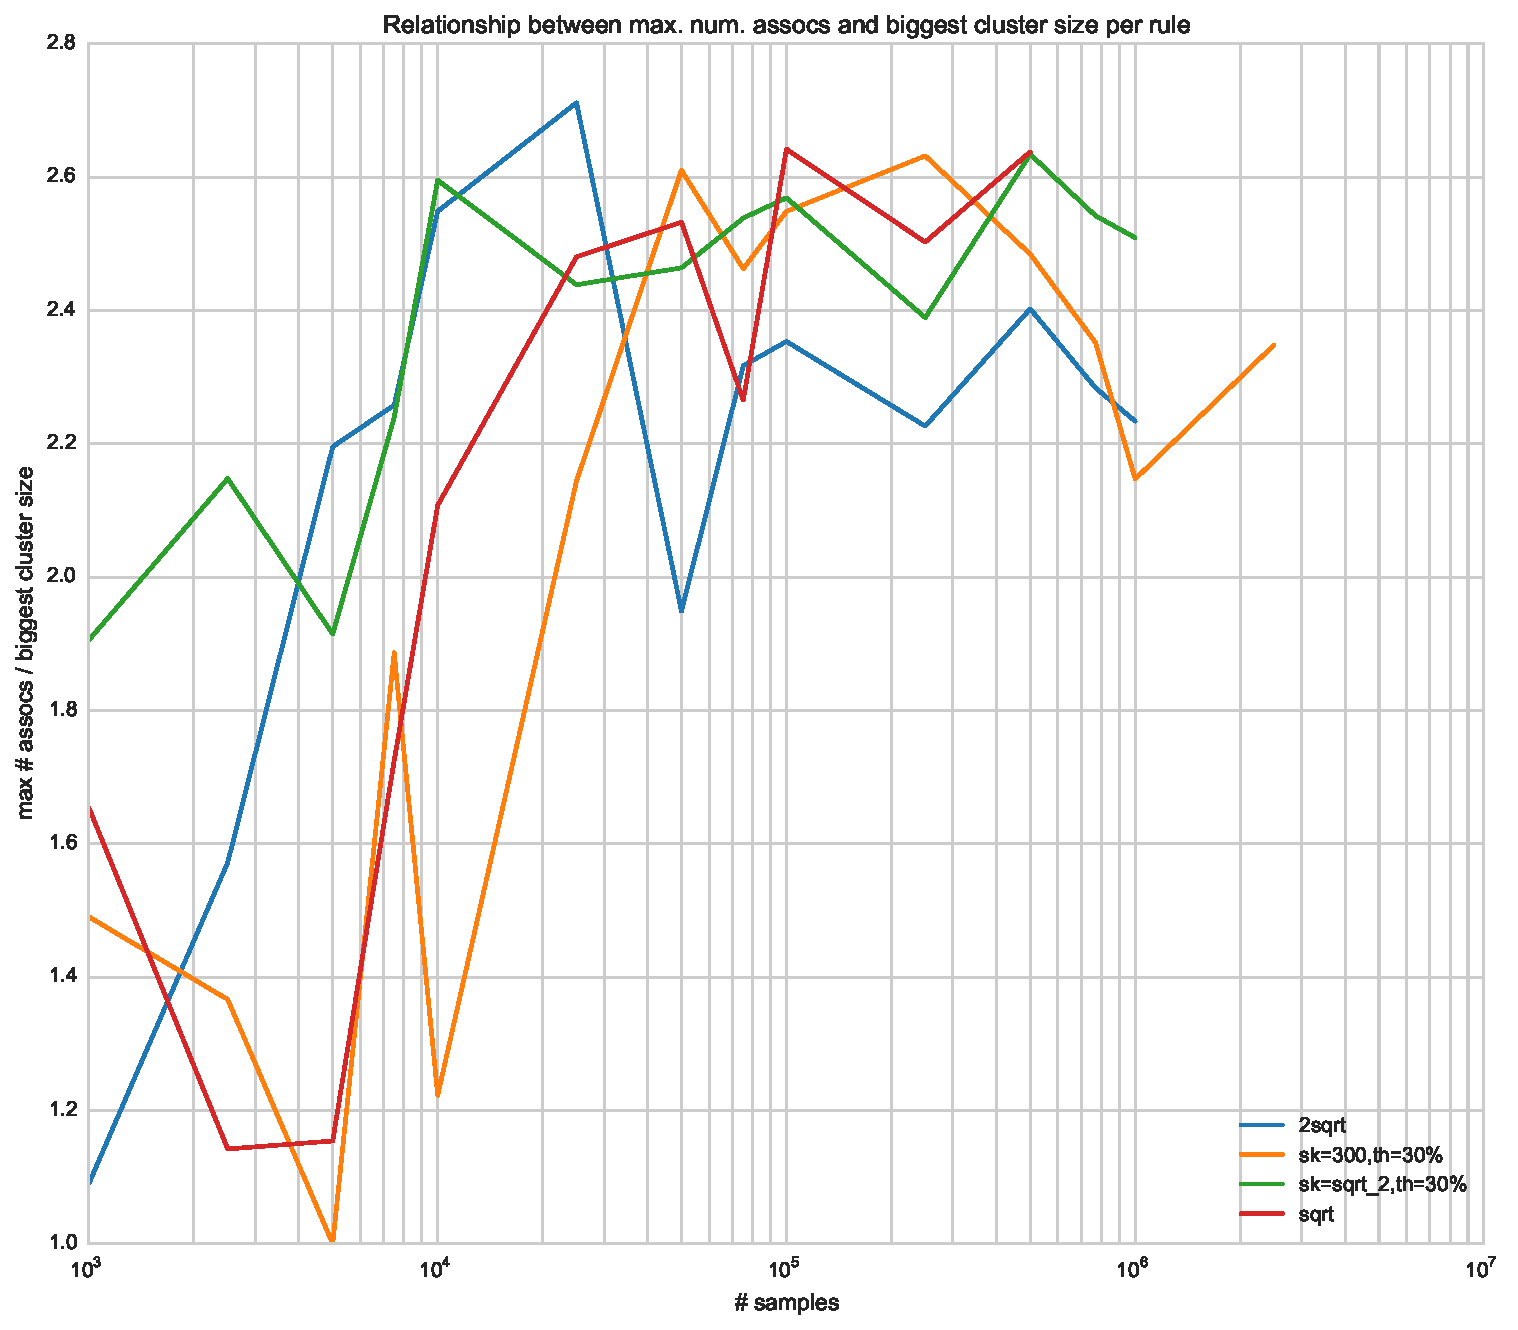
\includegraphics[width=0.6\textwidth]{{{results/eac/max_assoc_bgs}}}
    \caption{Maximum number of associations of any pattern divided by the number of patterns in the biggest cluster of the ensemble.}
    \label{fig:eac max assocs per bgs}
\end{figure}

However, the number of features of the used datasets is rather reduced.
It might be the case that this ratio would increase with the number of features, since there would be more degrees where the clusters might include other neighbors.
With this in mind, further studies ranging a wider spectrum of datasets should yield more enlightening conclusions or reinforce those presented here.

\subsection{Space complexity}

The previous section analyzed results related to the number of associations.
This is related to the space complexity of the different matrix formats, but does not present an accurate depiction of their complexity, mainly due to the data structures supporting the sparse formats.
The true space complexity of the formats can be observed in Figures \ref{fig:eac allocated density} and \ref{fig:eac mem density}.

As explained previously, the allocated space for the space formats is based on a prediction that uses the biggest cluster size of the ensemble.
This allocated space is usually more than what is necessary to store the total number of associations.
Furthermore, the CSR sparse format, on which the EAC CSR strategy is based, requires an array of the same size of the predicted number of associations.
This overhead may in fact make the sparse format pre-allocate more associations than actually are possible for some rules, as can be seen in Fig. \ref{fig:eac allocated density}.
Still, the allocated number of associations becomes a very small fraction compared to the \emph{full} matrix as the dataset complexity increases, which is typical case for using a sparse format.

\begin{figure}[hbt!]
    \centering
    \includegraphics[width=0.6\textwidth]{{{results/eac/allocated_density/sk=300}}}
    \caption{Allocated number of associations relative to the full $n^2$ matrix.}
    \label{fig:eac allocated density}
\end{figure}

The actual memory used, presented in Fig. \ref{fig:eac mem density}, follows roughly the same pattern.
Here, the data types used play a big role in the amount of memory that is required.
The associations can be stored in a single byte, since the number of partitions is usually less than 255.
This means that the memory used by the fully allocated formats is $n^2$ and $\frac{n(n-1)}{2}$ Bytes for the complete and condensed versions, respectively.
In the sparse formats, the values of the associations are also stored in an array of unsigned integers of 1 Byte.
However, an array of integers of 4 Bytes of the same size must also be kept to keep track of the destination pattern each association belongs to.
Besides, one other array of integers of 8 Bytes is kept but it is negligible compared to the other two arrays.
The impact of the data types can be seen for smaller datasets where the total memory used is actually significantly higher than that of the \emph{full} matrix.
It should be noted that this discrepancy is not as high for other rules as for $sk=300$.
Still, the sparse formats, and in particular the condensed sparse format, is preferred since the memory used for large datasets is a small fraction of would be necessary if using any of the fully allocated formats.

\begin{figure}[hbt!]
    \centering
    \includegraphics[width=0.6\textwidth]{{{results/eac/mem_density/sk=300}}}
    \caption{Memory used relative to the full $n^2$ matrix.}
    \label{fig:eac mem density}
\end{figure}

\subsection{Accuracy}

Finally, the accuracy of each solution was measured and is presented in Fig. \ref{fig:eac accuracy}.
The number of clusters of the final solutions was determined by the lifetime method.
The accuracy was the same for all rules and for all matrix formats in each dataset, except in the beginning were the $sk=300$ produces bad results due to the ensemble having partitions with a number of clusters inferior to the real number of clusters.
Still, the $sk=300$ rule is the one presented because it spans a wider spectrum of datasets.
When two classes are overlapping, the lifetime method typically interprets them as being the same class.
In the beginning, there are only two overlapping Gaussians, explaining the accuracy of roughly $84\%$.
As more patterns are added to the datasets, the accuracy lowers to around $66\%$, since now 4 classes are overlapped in pairs.
There are two lows in accuracy around the $50\%$.
The first is due to a "bridge" between two classes by a couple of patterns that are not present in the surrounding datasets duo to sampling.
The last is duo to the same reason, since now more patterns are included in the dataset.

\begin{figure}[hbt!]
    \centering
    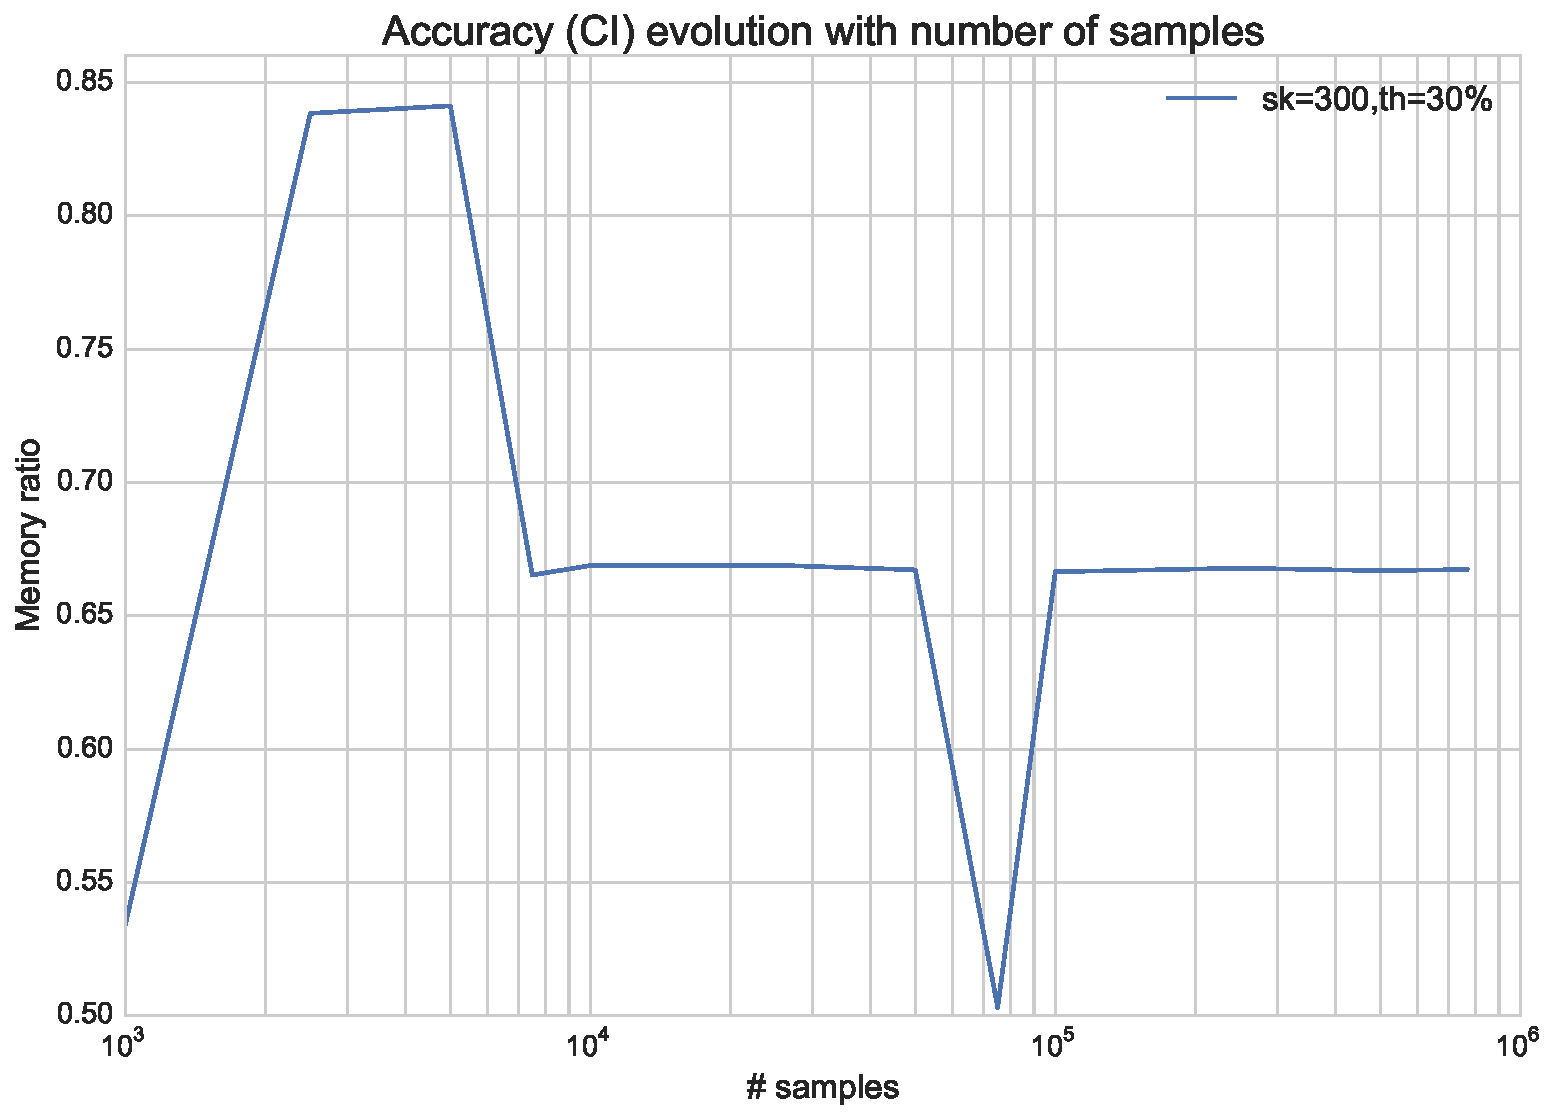
\includegraphics[width=0.6\textwidth]{{{results/eac/accuracy}}}
    \caption{Accuracy of the final clusterings as measured with the Consistency Index.}
    \label{fig:eac accuracy}
\end{figure}


\begin{table}[h]
\centering
\caption{Execution times for real-world large datasets.}

\begin{tabular}{llrrrrr}
\toprule
{} & dataset alias &  \# patterns &  \# features &  Production [sec] &  Combination [sec] &  Recovery [sec] \\
\midrule
0 &       PHYACT 1 &              441568 &                  30 &      2158.694059 &        123.858485 &      19.765186 \\
1 &       PHYACT 2 &              359170 &                  30 &      1477.346136 &         98.866711 &      15.796466 \\
\bottomrule
\end{tabular}



\label{tab:eac rules}
\end{table}

\section{Performance on real world datasets}

The proposed EAC method was tested on real world datasets.
Large real world datasets appropriate for clustering were hard to find freely available.
The datasets used are aimed at other Machine Learning analysis, such as classification or regression.
For this reason, the presented results are focused on performance.

\begin{table}[h]
\centering
\caption{Execution times for real-world large datasets. P and F refer to the number of patterns and features. P, C and R times refer to the production, combination and recovery times.}

\begin{tabular}{llrrrrr}
\toprule
dataset alias &  \# P &  \# F &  P time [s] &  C time [s] &  R time [s] \\
\midrule
PHYACT 1 \cite{Lichman:2013}.&              441568 &                  30 &      2158.69 &        123.85 &      19.76 \\
PHYACT 2 \cite{Lichman:2013}.&              359170 &                  30 &      1477.34 &         98.86 &      15.79 \\
% KDD99 &             2449216 &                  41 &     10284.166381 &  not possible to run because the bgs was 964287... &            NaN \\
esopH \cite{yuk13oro}        &                 136127 &                   2 &        17.94 &  35.15 &       3.95 \\
diabetes \cite{strack2014impact,Lichman:2013}&              101766 &                  41 &       188.56 &  33.79 &       5.07 \\
\bottomrule
\end{tabular}


\label{tab:eac rules}
\end{table} % EAC RESUTLS
%!TEX root = Thesis.tex

\section{Quantum Clustering}

This section presents performance and accuracy results of Quantum K-Means and Horn and Gottlieb's algorithm.
All results were obtained using machine Alpha.

\subsection{Quantum K-Means}

The testing was aimed at benchmarking both accuracy and speed.
The input used was synthetic data, namely, Gaussian mixtures with variable cardinality and dimensionality.

The tests were performed using 10 oracles, a qubit string length of 8 and 100 generations per round.
The classicalK-Means was executed using the \emph{k-means++} centroid initialization method to make for a fairer comparison, since QK-Means also has some computational cost in the beginning of the algorithm.
Since QK-Means executes a classical K-Means for each oracle each generation, the performance results for K-Means alone refer to $num.oracles \times num.generations \times factor$ runs, where $factor$ is an adjustable multiplier.
Each test had 20 rounds to allow for statistical analysis of the results.

All tests were done with 6 clusters (natural number of clusters).
Two tests were done with the two dimensional dataset: one with a $factor=1.10$ (increase initializations by $10\%$) and another with $factor=1$.
These tests will be called T1 and T2, respectively.
The test done with the six dimensional dataset (T3) used $factor=1.10$.

% table in csv format available in resource directory -->
Performance results are presented in Table \ref{tab:qkmeans times}.
The mean computation time of classical K-Means is an order of magnitude lower than that of QK-Means.
However, the solution chosen in classical K-Means was the one with lowest sum of squared euclidean distances of points to their attributed centroid.
To analyze the influence of the Davies-Bouldin (DB) index, it was computed on all classical K-Means solutions and used as the criteria to choose the best solution.
When this is done, we can see that the total time of classical K-Means is actually higher that that of QK-Means in T1 and T3, but this is only due to the 1.10 multiplier on the number of initializations.
In T2, the computation times become very similar with only a 2\% difference between these two variants.
Results show that most computational cost (88\% on T1) lies on the evaluation of the solutions obtained from each oracle, i.e. computing the DB index.
This is a costly but necessary step in this algorithm.

\begin{table}[h]
\centering
\caption{Timing results for the different algorithms in the different tests. Fitness time refers to the time that took to compute the DB index of each solution of classical K-Means. All time values are the average over 20 rounds and are displayed in seconds.}
\begin{tabular}{llrrrr}
\toprule
\textbf{Dataset}               & \textbf{Algorithm} & \textbf{Mean} & \textbf{Variance} & \textbf{Best} & \textbf{Worst} \\
\midrule
\textbf{T1}                    & QK-Means           & 62.02642975   & 0.077065212       & 61.620424     & 62.579969      \\
\textbf{bi36}                  & K-Means            & 6.4774672     & 0.002501651       & 6.352554      & 6.585451       \\
\textbf{}                      & K-Means + fitness  & 70.2238286    & 0.022223755       & 69.889105     & 70.548572      \\
\textbf{}                      & fitness            & 63.7463614    & 0.019722105       & 63.536551     & 63.963121      \\
\midrule
\textbf{T2}                    & QK-Means           & 64.22347165   & 0.056559152       & 63.807367     & 64.807373      \\
\textbf{bi36 noFactor}       & K-Means            & 5.71167475    & 0.004903253       & 5.581391      & 5.877091       \\
\textbf{}                      & K-Means + fitness  & 62.7021533    & 0.066919692       & 63.417207     & 62.180021      \\
\textbf{}                      & fitness            & 56.99047855   & 0.062016439       & 56.59863      & 57.540116      \\
\midrule
\textbf{T3}                    & QK-Means           & 74.4917966    & 0.067688312       & 74.12105      & 74.976446      \\
\textbf{sex36}                 & K-Means            & 8.291648      & 0.007015777       & 8.160859      & 8.426203       \\
                               & K-Means + fitness  & 72.36315915   & 0.05727269        & 71.856457     & 73.031841      \\
                               & fitness            & 64.07151115   & 0.050256913       & 63.695598     & 64.605638      \\
\bottomrule                           
\end{tabular}
\label{tab:qkmeans times}
\end{table}

DB index results are presented in Table \ref{tab:qkmeans DB}
These results show that the quality of the solutions from K-Means and QK-Means do not differ significantly on these data sets.
The results presented before steered the direction of the analysis to a "fairer" comparison.
Yet, the main requirement for the target application of this algorithm is speed.
In this regard, it is several orders of magnitude slower than the classical K-Means, since the K-Means performance results refer to many runs.
This, allied with the fact that the quality of the solutions does not differ much in the two algorithms and the fact that good quality is not necessary in the target application, makes the use of this algorithm prohibitive in the EAC context.

\begin{table}[h]
\centering
\caption{All values displayed are the average over 20 rounds, except for the Overall best which shows the best result in any round. The values represent the Davies-Bouldin fitness index (low is better).}
\begin{tabular}{llrrrr}

\toprule

\textbf{Dataset} & \textbf{Algorithm} & \textbf{Best} & \textbf{Worst} & \textbf{Mean} & \textbf{Variance}  \\
\midrule
\textbf{T1}      & QK-Means           & 15.42531927   & 32.29577426    & 19.94704511   & 21.23544567         \\
\textbf{}        & K-Means            & 15.42531927   & 25.44913817    & 16.25013365   & 1.216919278         \\
\midrule
\textbf{T3}      & QK-Means           & 22.72836641   & 65.19984617    & 36.10699242   & 78.14043743         \\
\textbf{}        & K-Means            & 22.71934191   & 46.72231967    & 26.18440481   & 22.96730826        \\
\bottomrule
\end{tabular}
\label{tab:qkmeans DB}
\end{table}





% \subsubsection{QK-Means details}

% Here we’ll analyse a bit what’s happening within each QK-Means execution. One would expect for the population’s fitness variance to decrease over the generations, as the probabilities for previous known solutions increase and are therefore more likely to reappear. The convergence of the population mean would also be expected to decrease for the same reason. However, experimental (Fig. \ref{fig:db_index_mean_t2} and \ref{fig:db_index_var_t2}) results don’t suggest any of these expectations (the results of T1 and T3 suggest the same). This may be due to low number of generations or simply because the random generation of initial centroids isn’t influenced enough by the qubit probabilities.


% \begin{figure}[hbtp]
% \centering
% 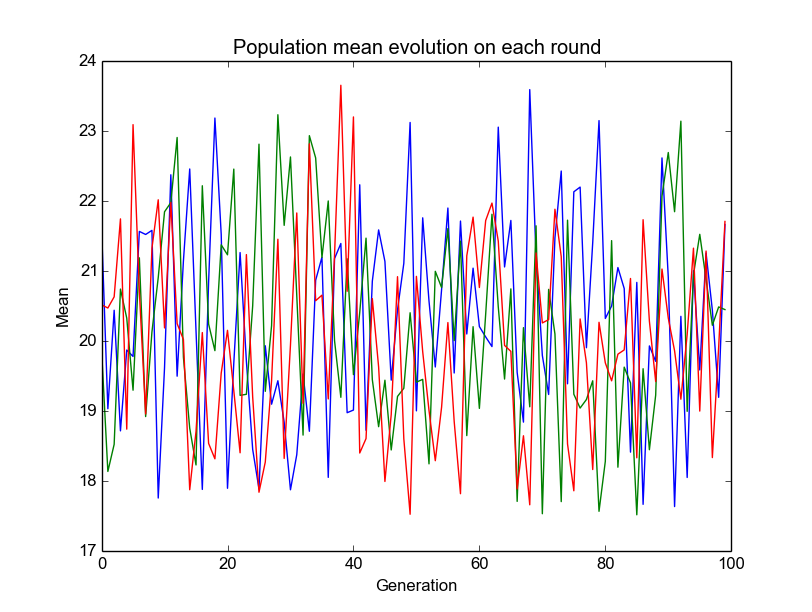
\includegraphics[scale=0.5]{QK_Means/img/bi_nofactor_mean.png}
% \caption{DB index mean of the population in T2. Only 4 rounds represented.}
% \label{fig:db_index_mean_t2}
% \end{figure}

% \begin{figure}[hbtp]
% \centering
% 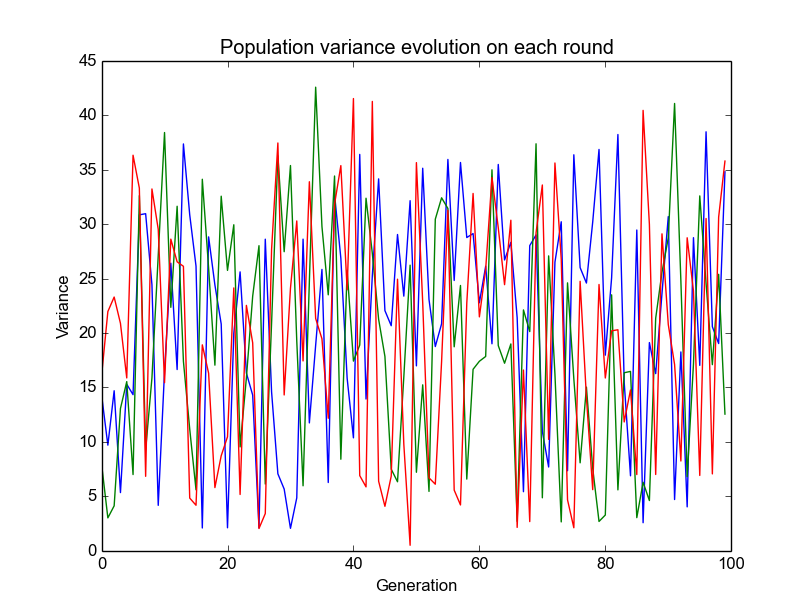
\includegraphics[scale=0.5]{QK_Means/img/bi_nofactor_var.png}
% \caption{DB index variance of the population in T2. Only 4 rounds represented.}
% \label{fig:db_index_var_t2}
% \end{figure}


% Analysing the evolution of the DB index of the best solution over the generations (Fig. \ref{fig:qk_db_index_best_evo_t2} and \ref{fig:qk_db_index_best_evo_t3}) gives some insight on the rate of convergence. In both tests it is clear that the best solution is often reached in a quarter of the total generations. More detail can be seen in the Table \ref{tab:db_index_t1_t3}.

% \begin{figure}[hbtp]
% \centering
% 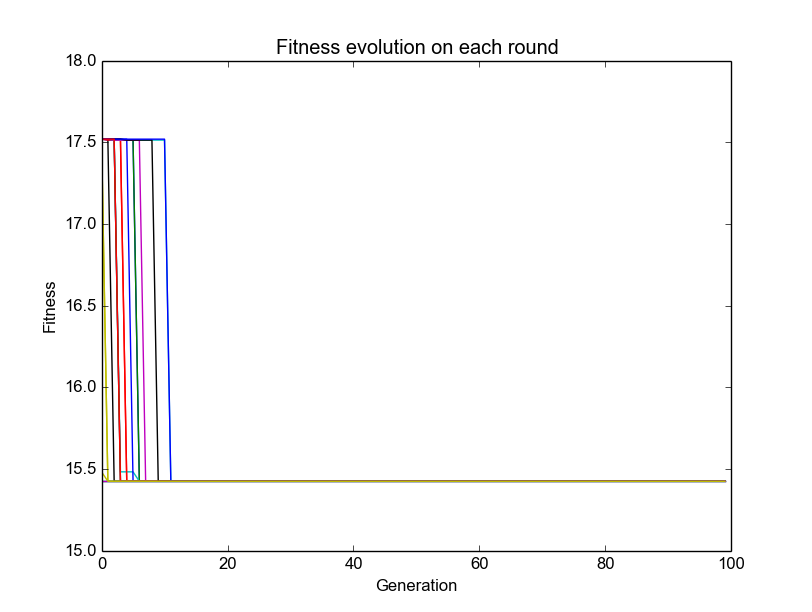
\includegraphics[scale=0.5]{QK_Means/img/bi_nofactor_evo.png}
% \caption{DB index of best solution in T2.}
% \label{fig:qk_db_index_best_evo_t2}
% \end{figure}


% \begin{figure}[hbtp]
% \centering
% 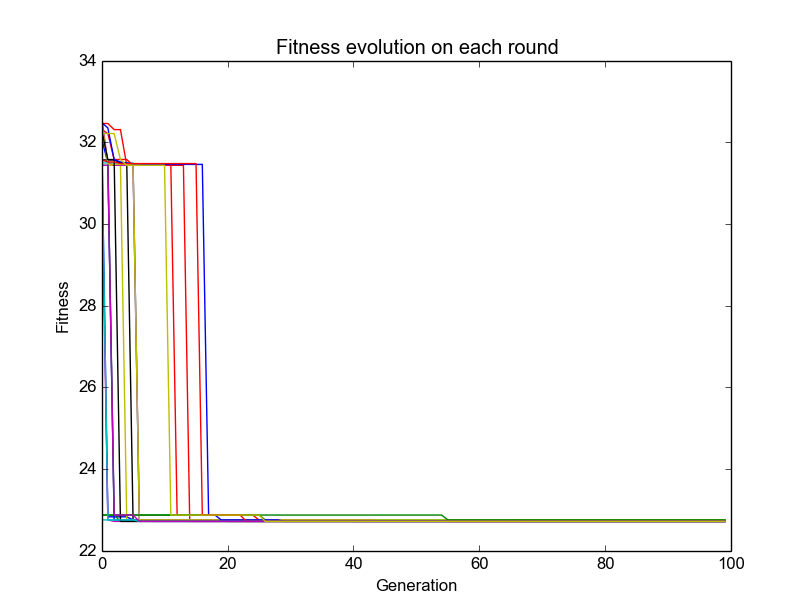
\includegraphics[scale=0.5]{QK_Means/img/sex_evo.png}
% \caption{DB index of best solution in T3.}
% \label{fig:qk_db_index_best_evo_t3}
% \end{figure}

% % table in csv format available in resource directory -->

% \begin{table}[h]
% \centering
% \caption{The values represent generations.}

% \begin{tabular}{lllll}

% \toprule
% \textbf{Test} & \textbf{Mean} & \textbf{Variance} & \textbf{Best} & \textbf{Worst} \\
% \midrule

% \textbf{T1}   & 17.25         & 70.2875           & 3             & 33             \\
% \textbf{T3}   & 28.05         & 568.6475          & 2             & 90             \\ 
% \bottomrule
% \end{tabular}

% \label{tab:db_index_t1_t3}
% \end{table}




\subsection{Horn and Gottlieb's algorithm}



All data in this section refers to processing done in machine Alpha.
For measuring the performance of this algorithm, several mixtures of 4 Gaussians with different cardinality and dimensionality were produced.
Table \ref{tab:horn performance} presents the execution times for each of these data sets.
It can be seen that the execution time of this algorithm is rather high even for small data sets as the ones presented, since this algorithm is being analyzed with the goal of speed optimization.
More than 1 hour for a small data set such as $10 \: 000$ patterns is prohibitive for application in the EAC context.

\begin{table}[h]
\centering
\caption{Time of computation of \citet{Horn2001b} algorithm for a mixture of 4 Gaussians of different cardinality and dimensionality.}

\begin{tabular}{rrr}
\toprule
 Cardinality &  Dimensionality &     Time [s] \\
\midrule
          10 &               2 &     0.035382 \\
          10 &               3 &     0.411391 \\
          10 &               4 &     0.385114 \\
          10 &               5 &     0.429747 \\
         100 &               2 &     2.954650 \\
         100 &               3 &     3.322593 \\
         100 &               4 &     3.743720 \\
         100 &               5 &     4.143823 \\
        1000 &               2 &    52.840666 \\
        1000 &               3 &    60.293262 \\
        1000 &               4 &    68.225671 \\
        1000 &               5 &    81.523212 \\
       10000 &               2 &  3009.678259 \\
       10000 &               3 &  3418.342830 \\
       10000 &               4 &  3956.289064 \\
       10000 &               5 &  4918.185844 \\
\bottomrule
\end{tabular}

\label{tab:horn performance}
\end{table}


In spite of its computational complexity, the accuracy of the algorithm was tested on the Iris and Crab data sets.
The Iris data set has 150 patterns, 4 features and 3 classes where 2 are overlapping.
The Crab data set has 200 patterns, 5 features and 4 classes where 2 pairs of classes are overlapping.
Principal Component Analysis (PCA) was applied to both data sets before clustering.
An accuracy as high as $86\%$ was obtained for the Iris data set when using the first and second principal components (PC), and as high as $82\%$ when using all PCs.
For the Crab data set an accuracy of $81.5\%$ was obtained for the second and third PCs (PCs chosen to reproduce the results of the original source of the algorithm), $63\%$ when using all PCs.
However, when applied to the unprocessed data the accuracy was only $34\%$ .


%TODO
%Put in accuracy results for crab,iris and gaussian mixtures  
%Put in timing results


% The accuracy of this algorithm was tested with real world datasets, namely, the crab and iris datasets available at the UCI Machine Learning Repository.

% %TODO add ref for repository -->

% \subsection{Iris data}
% \label{sec:horn_iris}
% The iris dataset ([available at the UCI ML repository](http://archive.ics.uci.edu/ml/datasets/Iris)) has 3 classes each with 50 data points. There are 4 features. The data is preprocessed using Principal Component Analysis (PCA). The natural clustering can be observed in Fig. \ref{fig:iris_natural}. 

% % #TODO saved image from ipython -->

% \begin{figure}[hbtp]
% \centering
% 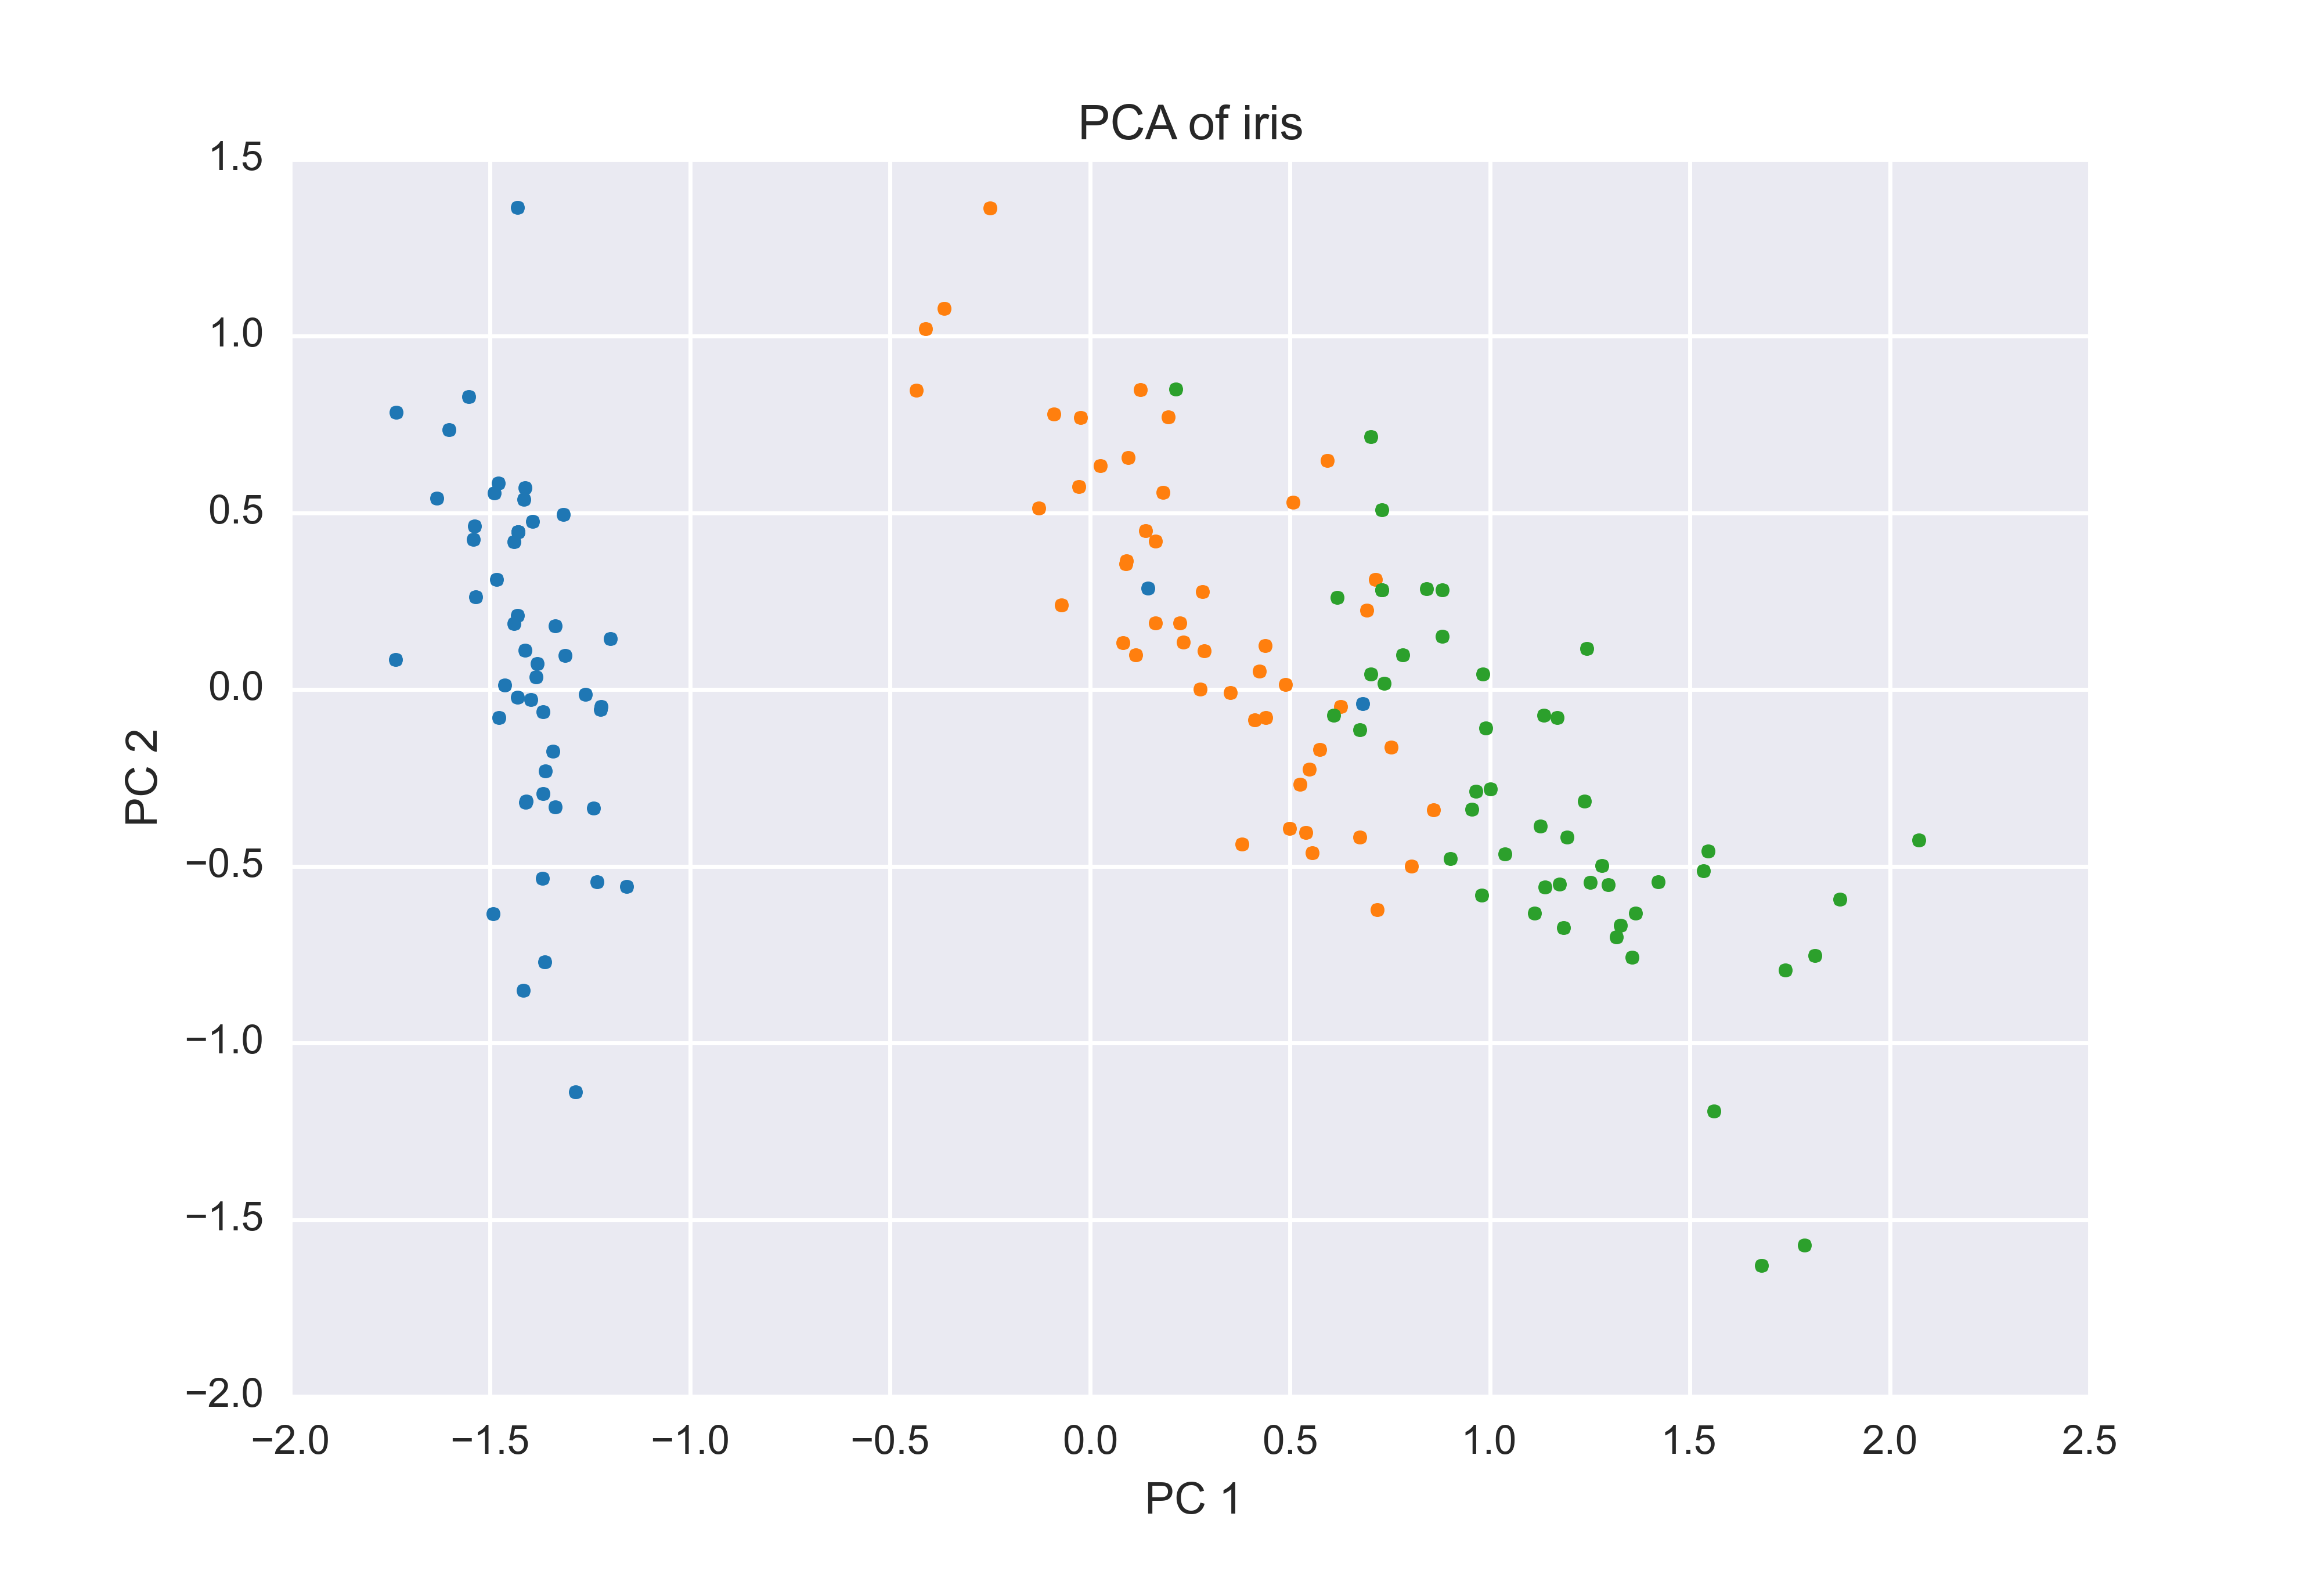
\includegraphics[scale=0.5]{Horn/img/iris_natural.png}
% \caption{Plot of the two first principal components (PC).}
% \label{fig:iris_natural}

% \end{figure}

% I chose $\sigma=\frac{1}{4}$ to reproduce the experiments in [3]. Only the first two PC are used here, which account for $95.8\%$ of the energy. The clustering results can be seen in Fig. \ref{fig:iris_2pc_cluster} and have an accuracy of 86\% computed with consistency index.


% \begin{figure}[hbtp]
% \centering
% 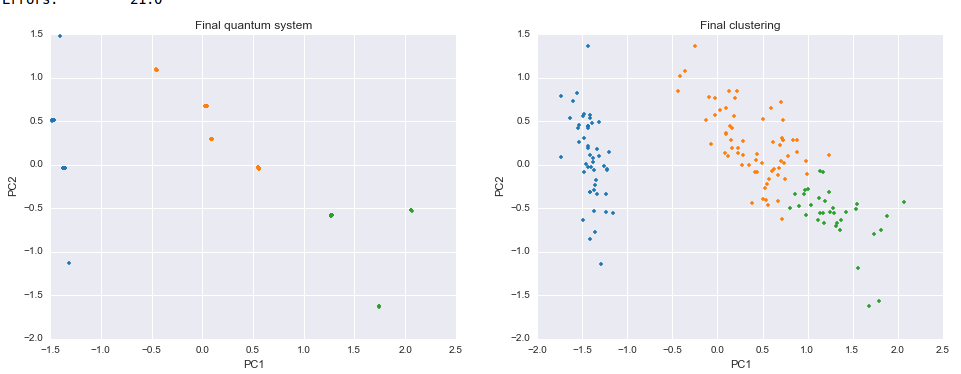
\includegraphics[width=\textwidth]{Horn/img/iris_2pc_cluster.png}
% \caption{Plots of the converged data data points and final clustering for 2 PC.}
% \label{fig:iris_2pc_cluster}

% \end{figure}

% For the sake of completeness, Fig. \ref{fig:iris_allpc_cluster} shows the clustering over all PCs. This solution has an accuracy of 82.67\% computed with consistency index.


% \begin{figure}[hbtp]
% \centering
% 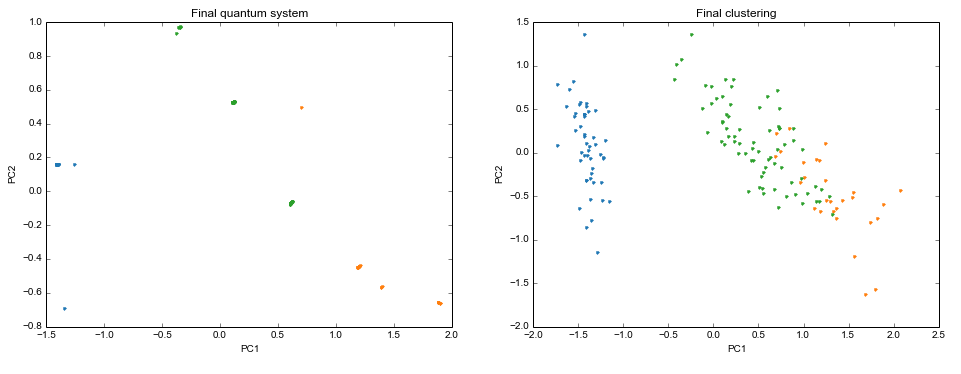
\includegraphics[width=\textwidth]{Horn/img/iris_allpc_cluster.png}
% \caption{Plots of the converged data data points and final clustering for all PC of Iris data.}
% \label{fig:iris_allpc_cluster}
% \end{figure}


% \subsection{Crab data}

% The crabs dataset has 200 samples and describes 5 morphological measurements on 50 crabs each of two colour forms and both sexes (total of 200 crabs), of the species Leptograpsus variegatus collected at Fremantle, Western Australia. After a preprocessing using PCA with covariance matrix and uncentred data, the dataset is represented in Fig. \ref{fig:crab_2pc_covar}.% #TODO add reference to dataset -->

% \begin{figure}[hbtp]
% \centering
% 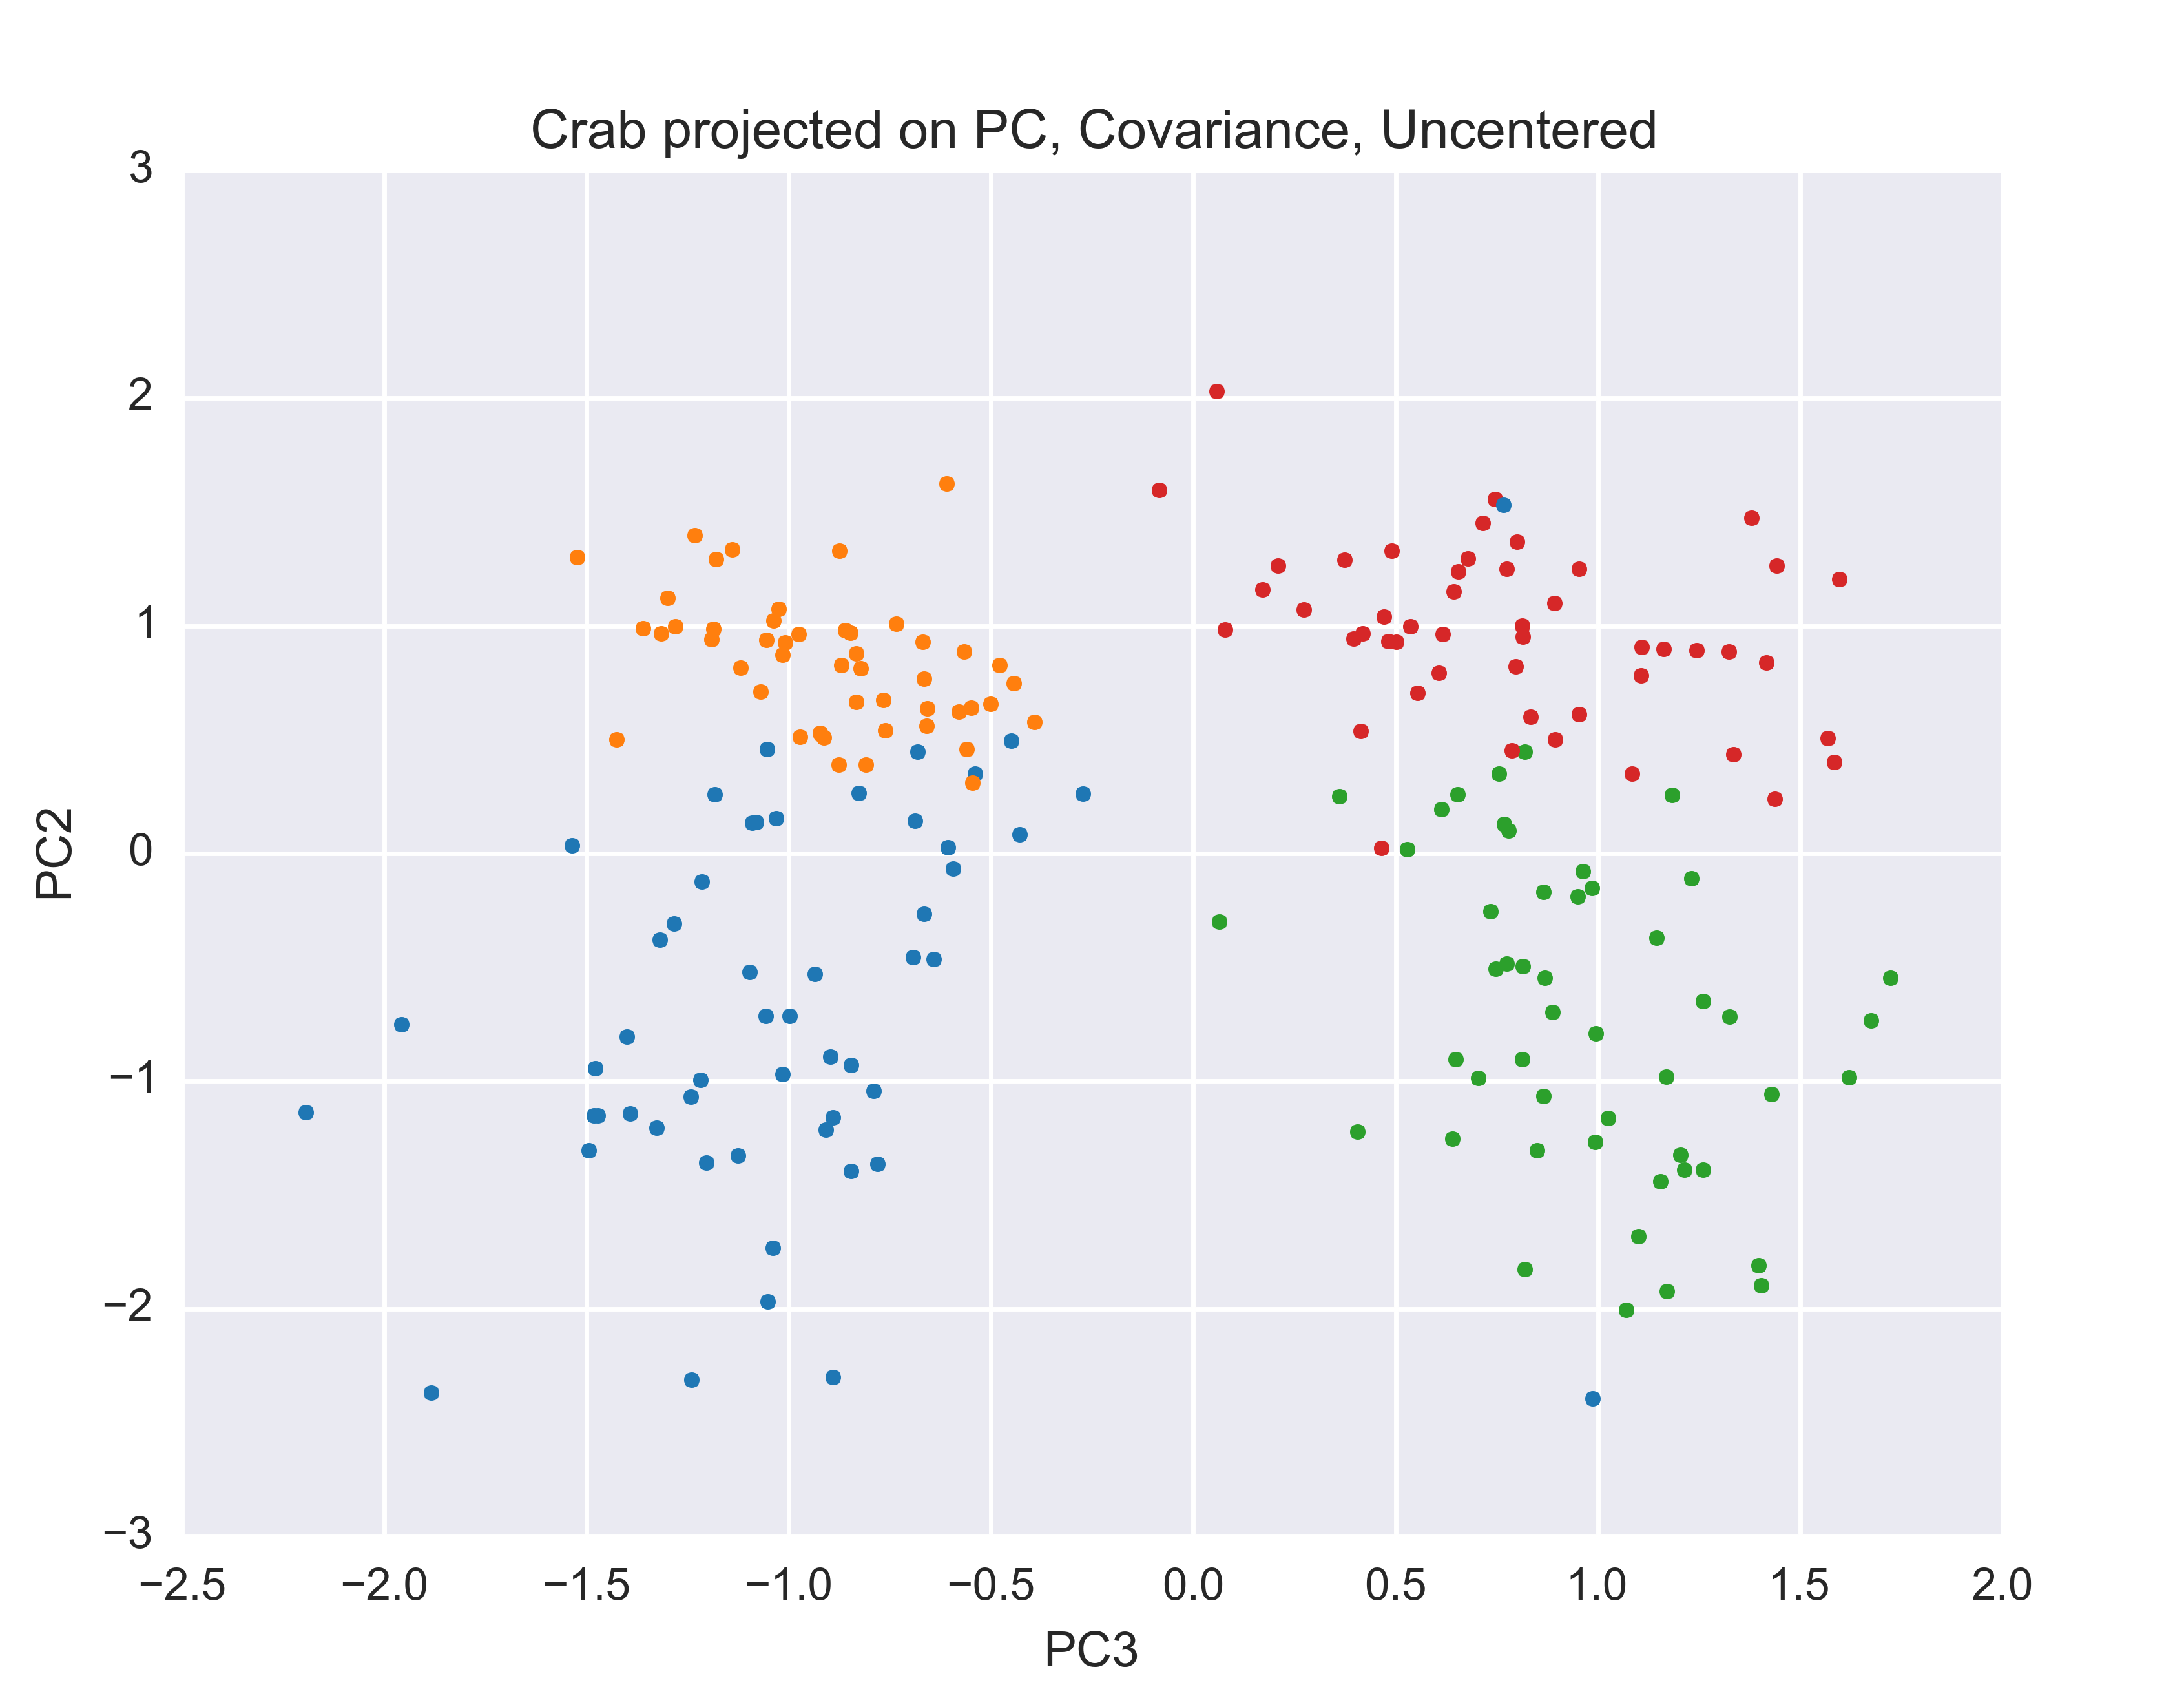
\includegraphics[scale=0.5]{Horn/img/crab_2pc_covar.png}
% \caption{Representation of the crab data projected over PC 2 and 3.}
% \label{fig:crab_2pc_covar}
% \end{figure}

% \begin{figure}[hbtp]
% \centering
% 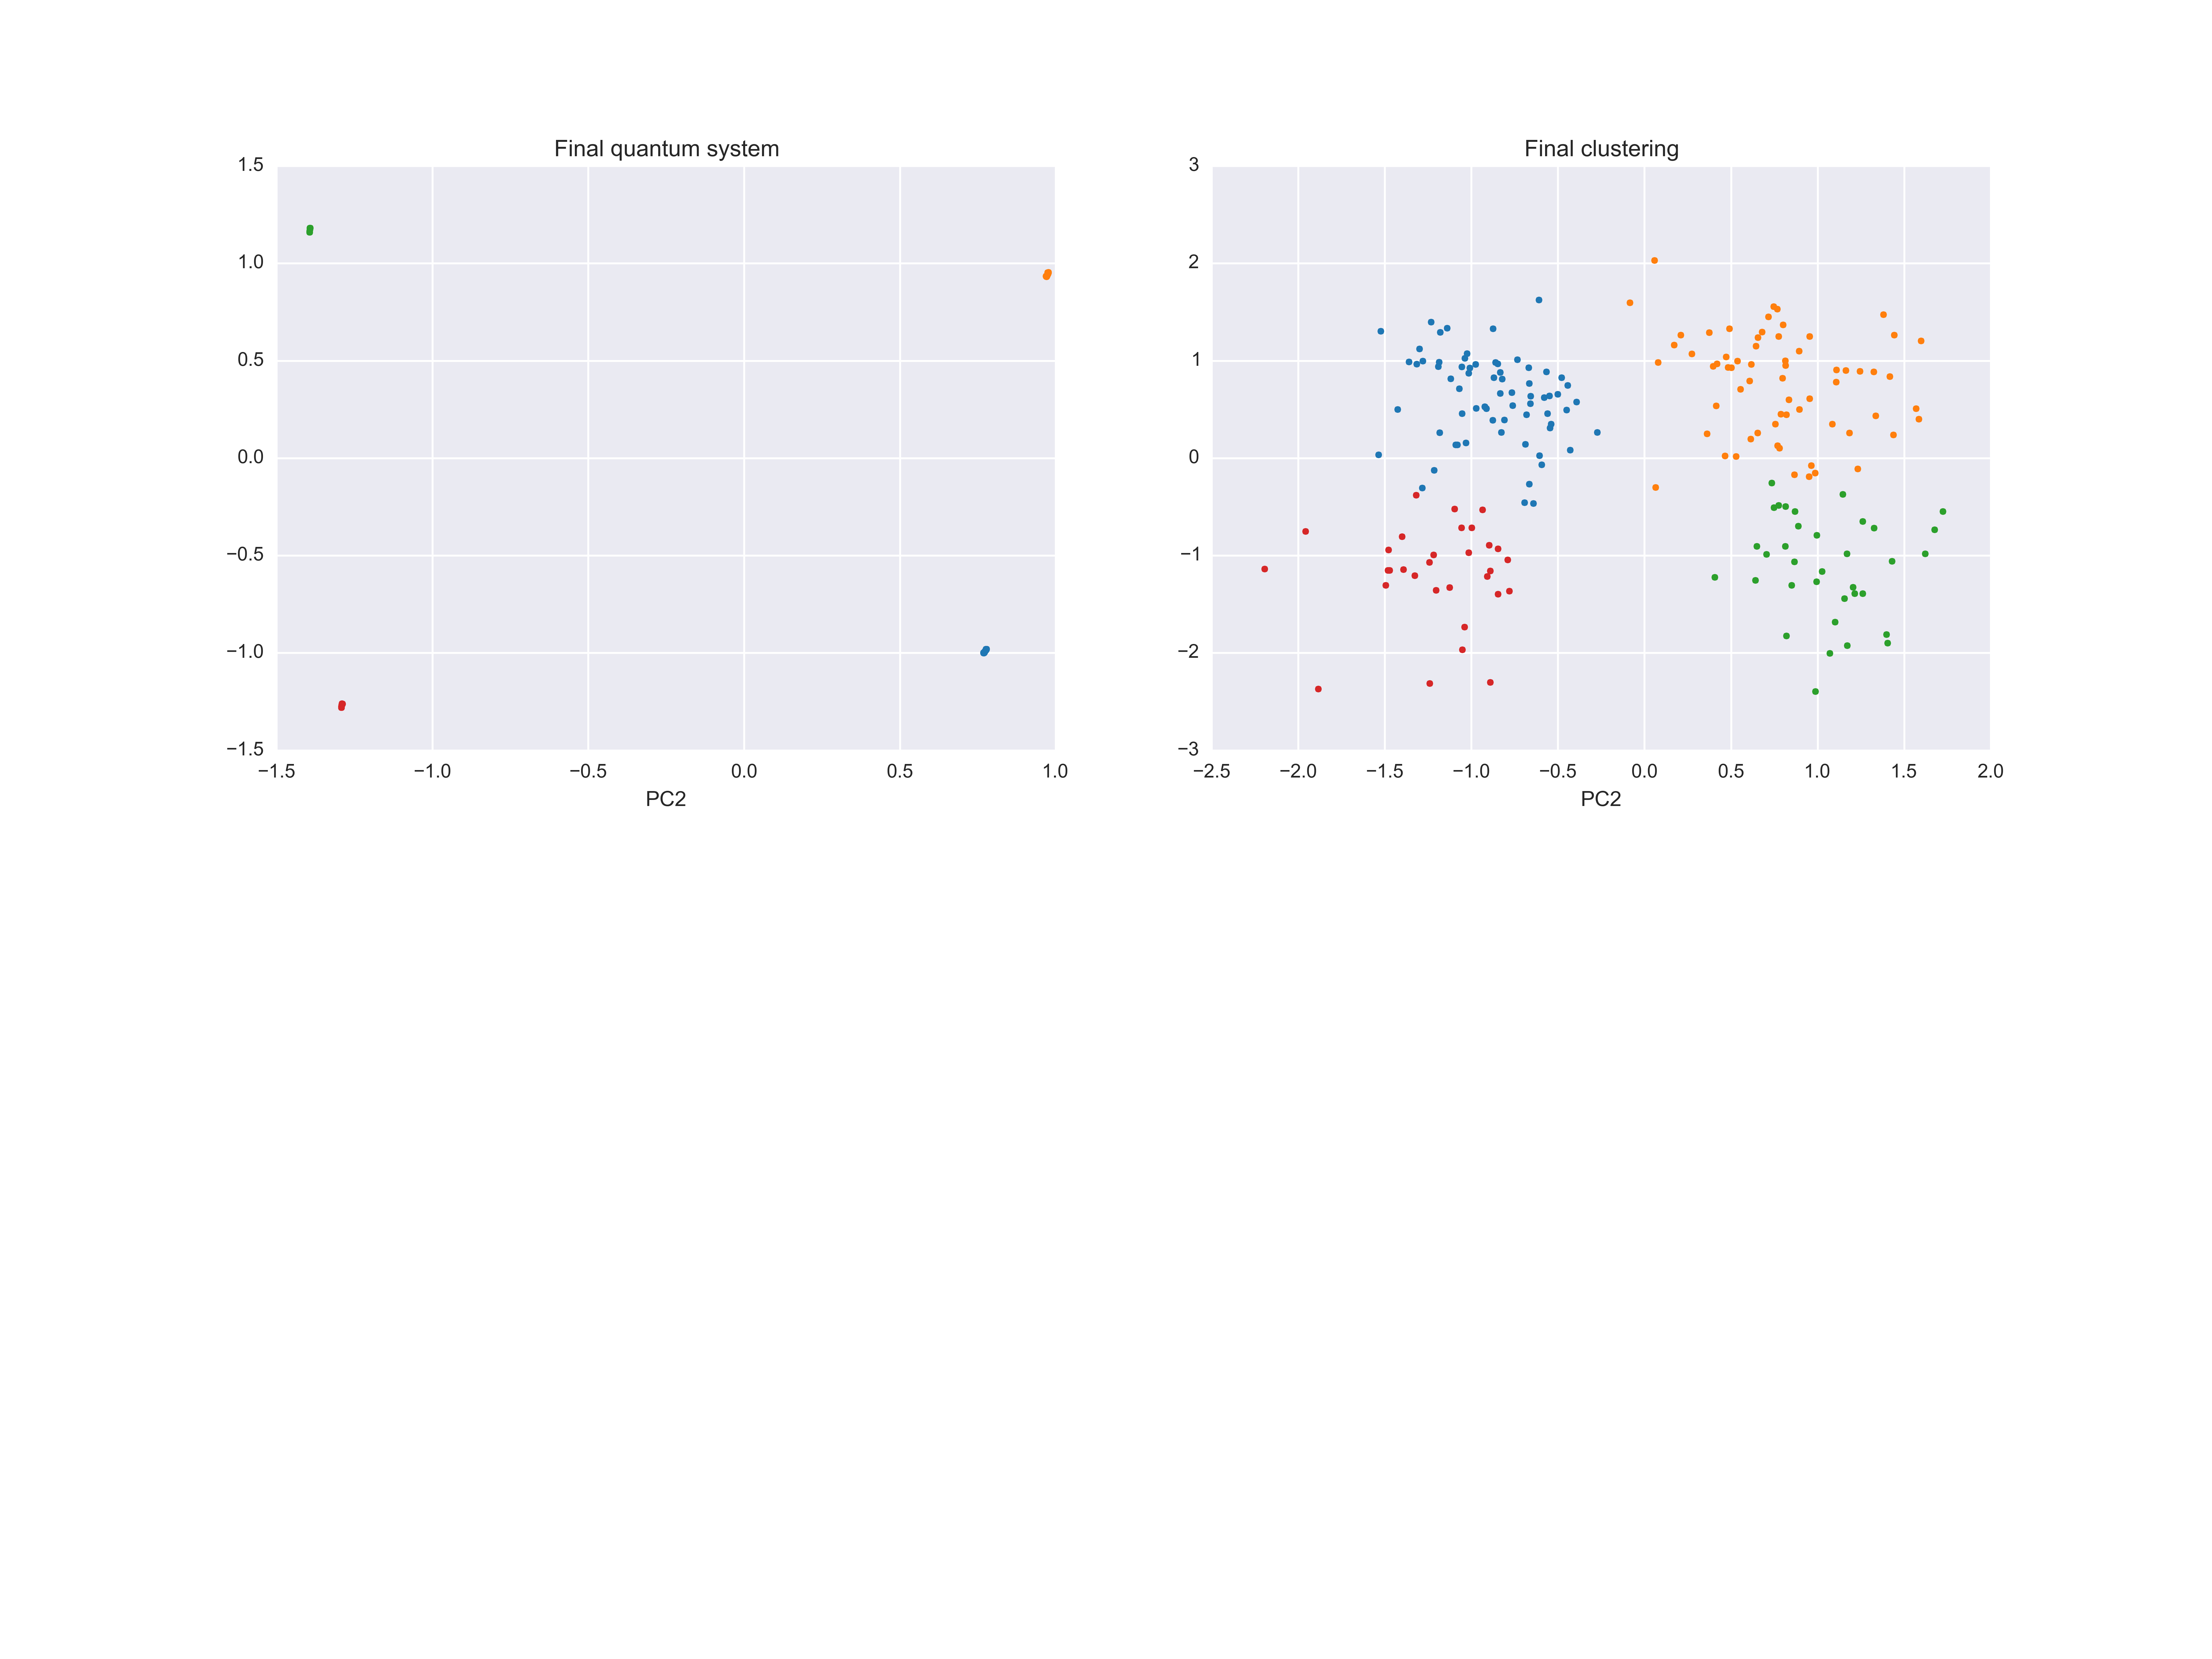
\includegraphics[width=\textwidth]{Horn/img/crab_2pc_covar_cluster.png}
% \caption{Representation of the crab data projected over PC 2 and 3.}
% \label{fig:crab_2pc_covar_cluster}
% \end{figure}

% \begin{figure}[hbtp]
% \centering
% 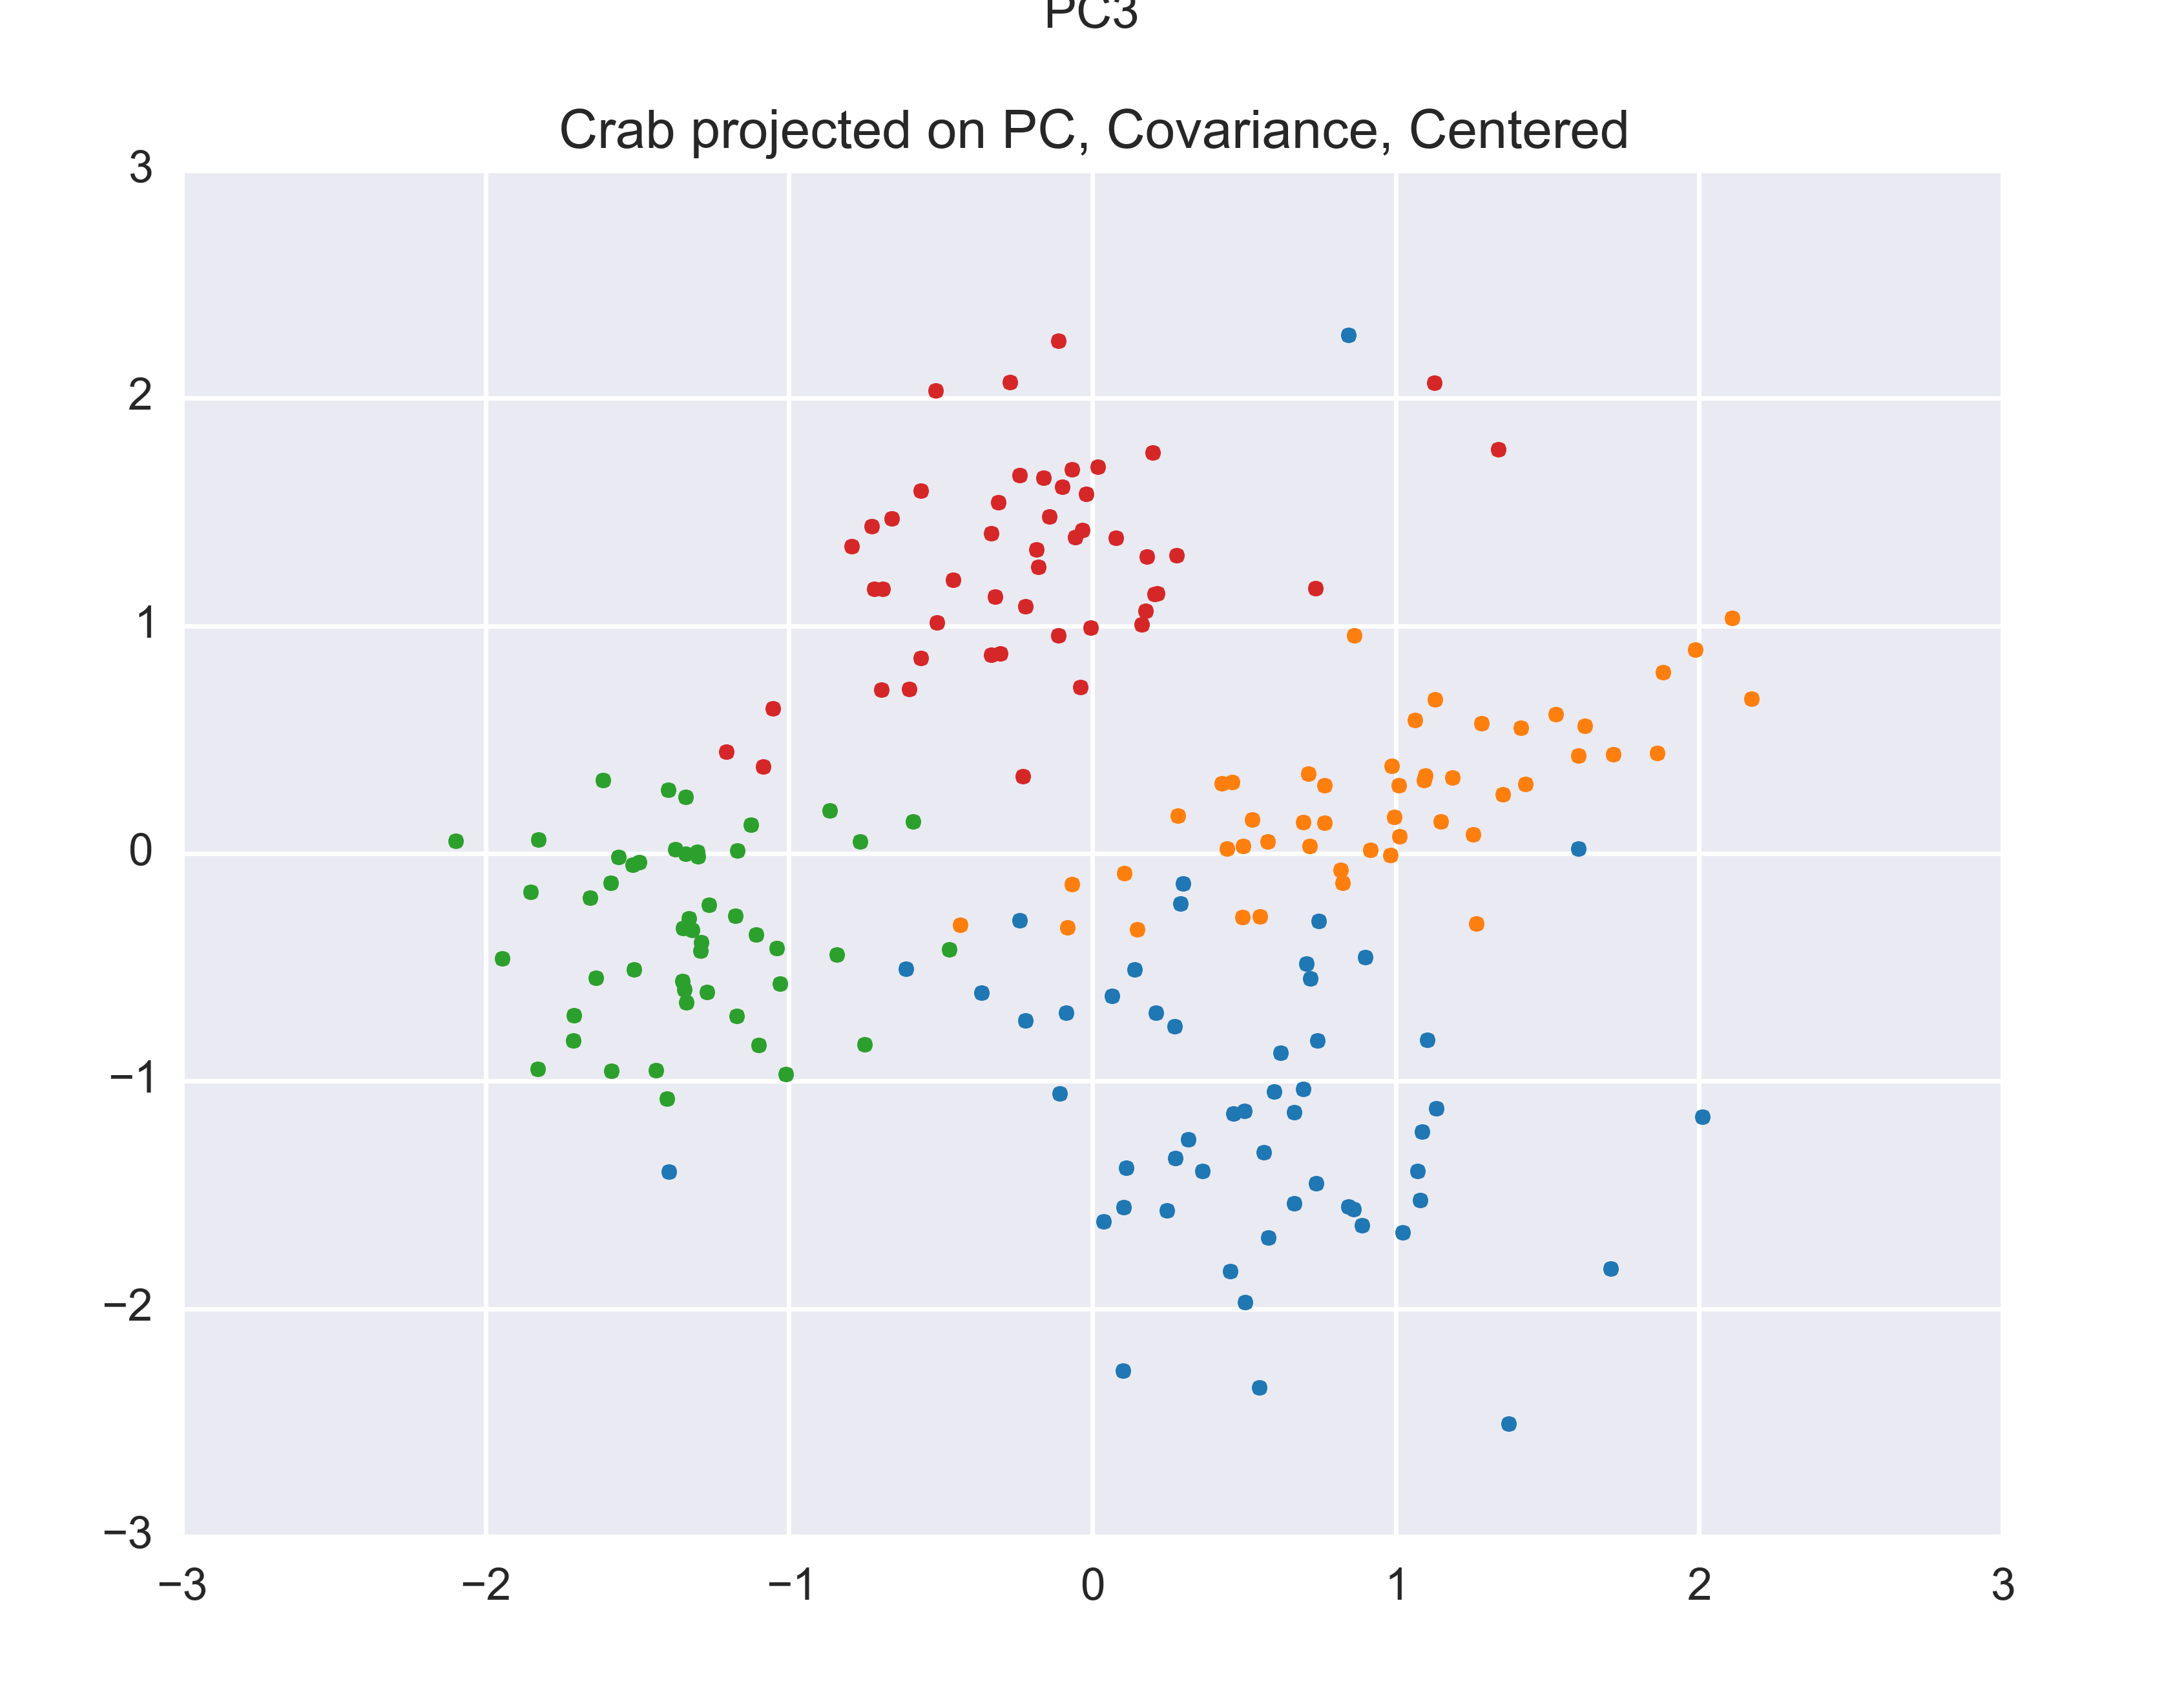
\includegraphics[scale=0.5]{Horn/img/crab_2pc_covar_centered.png}
% \caption{Representation of the crab data projected over PC 2 and 3.}
% \label{fig:crab_2pc_covar_centered}
% \end{figure}

% \begin{figure}[hbtp]
% \centering
% 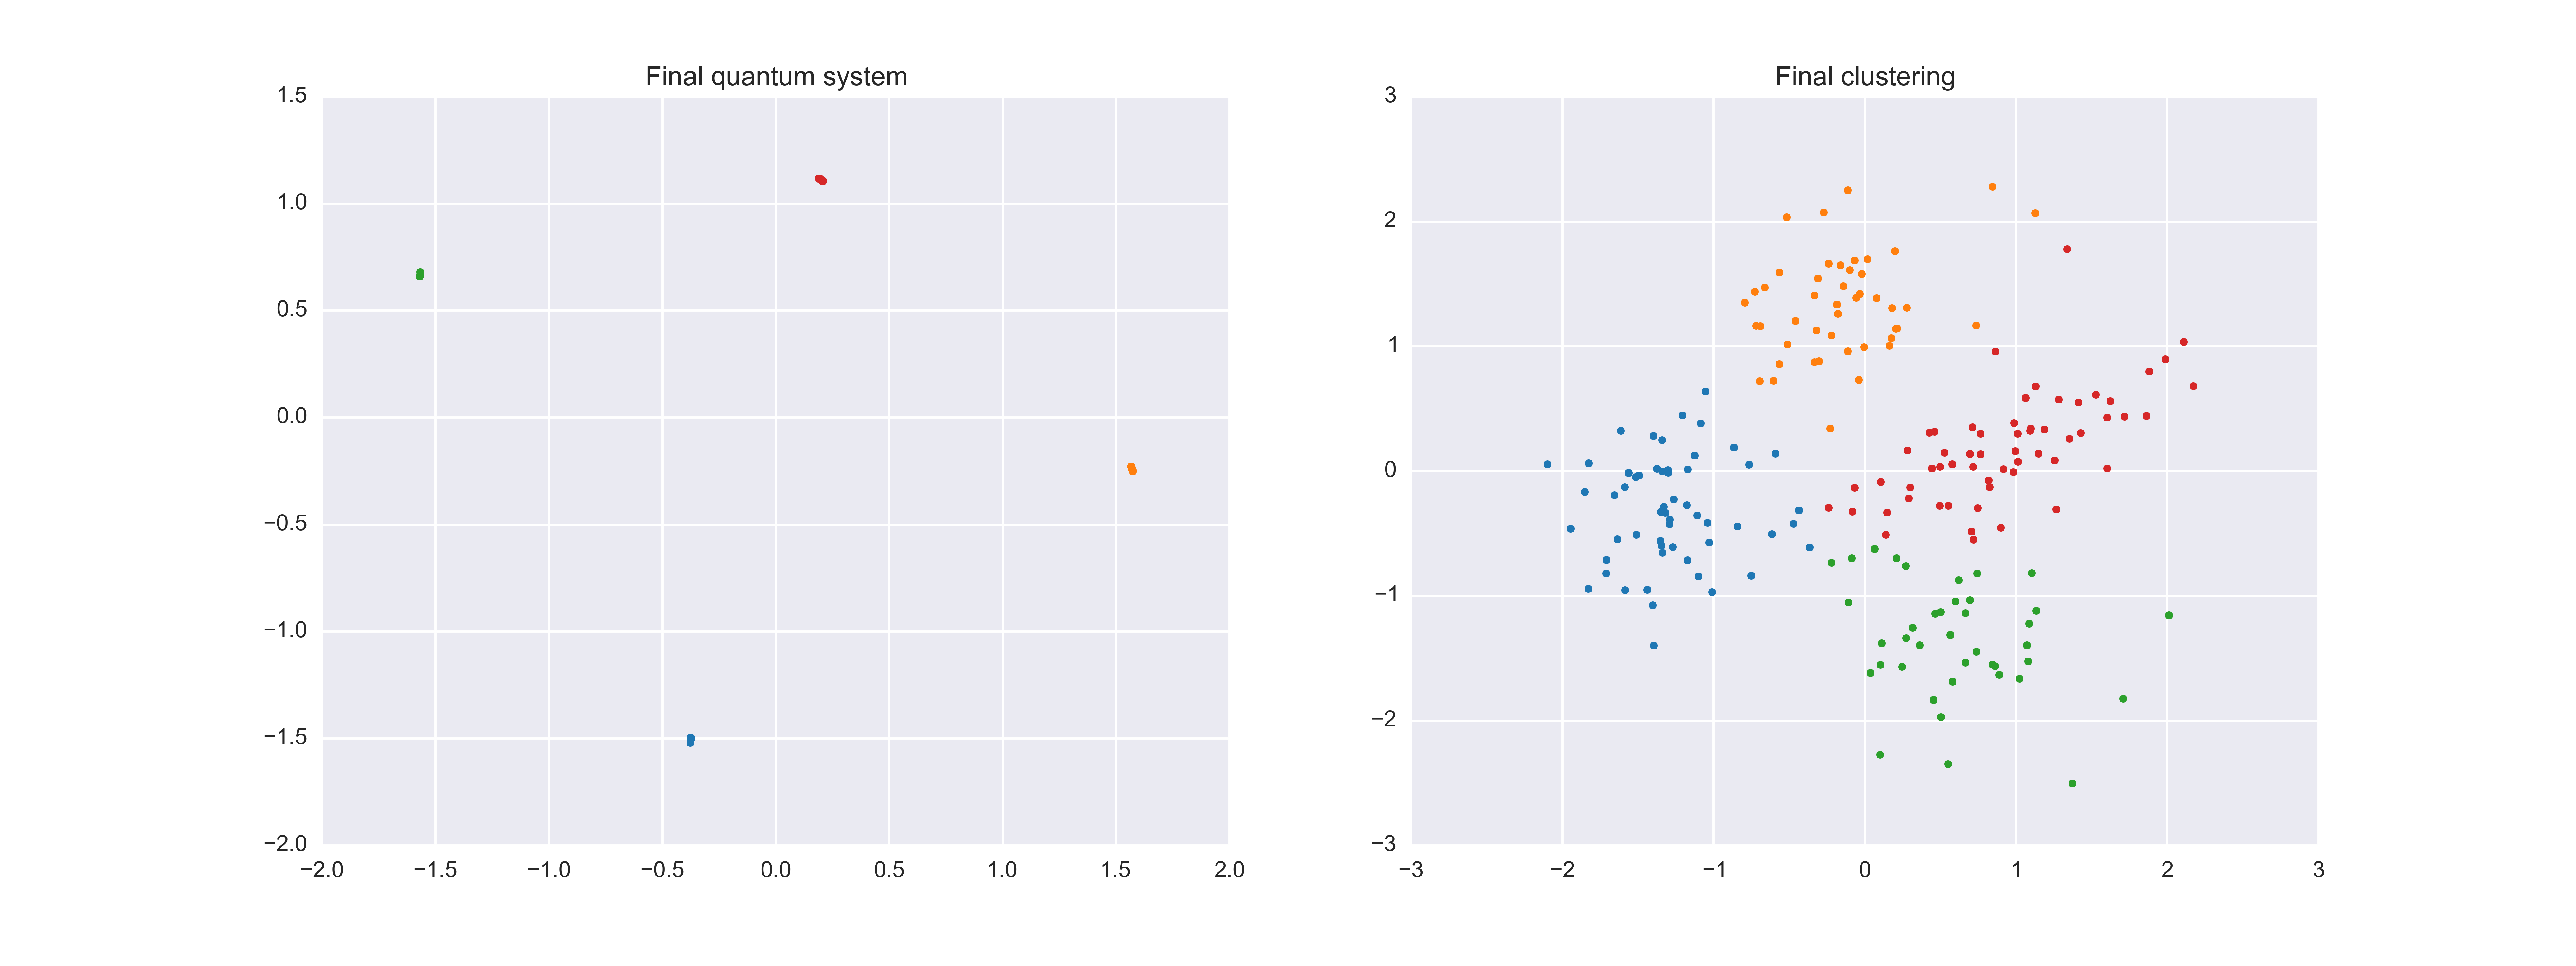
\includegraphics[width=\textwidth]{Horn/img/crab_2pc_covar_centered_cluster.png}
% \caption{Representation of the crab data projected over PC 2 and 3.}
% \label{fig:crab_2pc_covar_centered_cluster}
% \end{figure}


% Initial work aimed at reproducing results from [2], but lack of detail on the preprocessing used made it an harder task. Several preprocessings were used, namely whitening or not the data, centring it or not, using covariance versus correlation and different methods of computing the PCs through eigenvalue decomposition or Singular Value Decomposition (SVD). The closest representation to that of the [2] is the one if Fig. C1.


% %TODO finish crab

% Covariance uncentred consistency index = 0.815
% Covariance centred consistency index = 0.91

% all pc covariance uncentred consistency index = 0.63
% all dimensions original data consistency index = 0.34 % QUANTUM RESULTS